\chapter{DemVR: Exploring Shifting Sensitivities in a Hackathon for Dementia}
\label{DemVR}

\section{Introduction}
\label{sec:DemVRIntroduction}
In the previous chapter, I discussed two studies I conducted with people with dementia with Silverline Memories. Through these studies, I developed a set of VR and media experiences for families with dementia that engaged with the importance of personalisation; designing for being in the moment; placing equal importance on the different values in the ecology of care; and exploring ways for people with dementia to be actively involved in the research process. Through a reflective account, I describe the complexities I encountered in involving people with dementia in the participatory process. The reflections raise issues centring on the ethical challenges researchers face when planning and conducting dementia HCI research and uncertainty in how designers and developers can appropriate such participatory approaches to encourage the involvement of people with dementia.

In chapter four, I reflected on the challenges and training that went into moving from a developer skillset (through Computer Science undergraduate) to a user researcher skillset focused on working within sensitive settings. However, while I had the opportunity of taking time and building relationships with the families I was collaborating with, this is unlikely to be the case for developers or designers working in a more commercial space due to time constraints. This chapter builds an understanding of how designers and developers approach sensitive topics through their design process. One such space that brings together designers and developers to develop new paths to research, ideate and test software or products are hackathons \citep{kienzler_learning_2017}. Typically, hackathons have been known to target technical students who are willing to offer their time and technical skills in exchange for the opportunity to network with companies and learn new soft skills and new insights into areas they may have yet to explore \citep{olesen_what_2021}. In recent years, various domains have adopted hackathons to prioritise to responding to issues beyond the software or hardware skillsets of attendees. For instance, `civic hackathons' \citep{johnson_civic_2014} have aimed to improve citizen-government relationships through transparency and open data and events focused on `social good' \citep{ferrario_software_2014}. Within HCI, hackathon research has demonstrated useful cases for participation, learning, building and connecting people in communities of practice \citep{falk_olesen_10_2020, birbeck_self_2017, hou_hacking_2017, johnson_civic_2014}. However, such events pose challenges of longevity \citep{birbeck_self_2017}, compensation \citep{endrissat_hackathons_2018}, accessibility \citep{hope_hackathons_2019} and representation of the area for which attendees are designing \citep{toombs_hackerspace_2017}. 

To explore engagement with the topic of dementia, I ran a two-day hackathon called DemVR, which aimed to provide a space for participants to design novel use cases of shared VR experiences for people with dementia and their care partners. Much of dementia research emphasises the importance of relationships and sensitive design to support close and personal interactions. However, given that the approach requires long-term engagement between the researcher and participants, \added{this can result} in small participant pools. With the hopes of increasing accessibility for people with dementia, I ran the hackathon in two stages. The first was a pre-hackathon event, running over six weeks, where attendees, people with dementia and their care partners took part in short consultations via an online platform, Ideaboard, to share possible VR ideas. Following this engagement, I organised a two-day hackathon that invited designers, technologists and other makers to further develop their ideas with domain experts and people with dementia. While the event gained reasonable interest from designers, developers and students, the event struggled to involve and interest people with dementia and care partners to participate. The failure in representing people with dementia had multiple knock-on effects on teams' outputs that I describe in the findings. Building from these insights, the chapter ends with reflecting on the hackathon structure. Using dementia as a case example here, the chapter proposes alternative approaches for collaborative design events, community building through design and reification in design.

% The study covered in this chapter is currently being peer-reviewed in the TOCHI journal. The paper is co-authored by Dr. Sarah Foley, Dr. Daniel Lambton-Howard, Dr. Kyle Montague, Dr. Laura Booi, Sandra Hastings, Prof. David Kirk, and Dr. Kellie Morrissey. I was responsible for concept, study design, data collection, data analysis and writing of the paper. Co-authors supported the facilitation of the hackathon, and Dr. Kellie Morrissey, Dr. Sarah Foley and Dr. David Kirk provided feedback on the paper's writing and contribution.

% \section{Related work}
% \label{DemVR:RelatedWork}
% To provide context for the sensibilities informing the design of DemVR, I discuss the current approaches in designing for and with people with dementia and conclude the section by considering the challenges and opportunities of including such populations in public design events such as hackathons.

% \subsection{Learning about dementia through design}
% \label{DemVR:DementiaThroughDesign}
% Dementia is a neurodegenerative condition causing changes to cognitive ability and increasing reliance on social and physical care; bringing with it experiences of stigmatisation and subsequent social isolation  \citep{herrmann_systematic_2018}. Moving from an early, medicalised understanding of dementia as a process of decline and memory loss, recent social justice and rights-based responses to the experience of dementia have resulted in a more holistic understanding of the condition \citep{shakespeare_rights_2019}. This evolving understanding of dementia is mirrored in social and technological responses in research, which moved from early assistive technologies focusing on bridging a ‘cognitive gap’ \citep{mulvenna_supporting_2010}, to experience-centred design that fosters creative expressions of personhood \citep{morrissey_value_2017}, to more recent work on supporting wider social engagement with people with dementia \citep{foley_care_2019, lazar_safe_2019, welsh_ticket_2018}. Through the progression of understanding best practices for designing with and for people with dementia, HCI researchers have developed a series of approaches which centre relational interactions, as opposed to  engaging this population solely at the end of the design process,  e.g., by inviting participants for ‘user testing’ or ‘user evaluations’ \citep{brankaert_intersections_2019,schorch_designing_2016, vines_designing_2013}. However, by providing a more relational approach to our work, the researcher and participant are faced with different challenges. For instance, longer-term commitment to projects to support trust-worthy relationships between the researcher and participants \citep{hendriks_challenges_2014}; complex ethical considerations \citep{hornung_challenges_2016}; and the responsibility to take a caring and compassionate procedure to the research study \citep{balaam_emotion_2019}. 

% In response to the increase in multidisciplinary teams (often consisting of designers, developers, and researchers in the field) researchers have developed several toolkits and guides \citep{astell_using_2019, broderick2020theory,jais_evidence_2018} in an attempt to best guide the ways we involve and work with people with dementia.  For the majority, they have been provocative and useful toolkits that provide researchers the knowledge and insight into the best ways to involve people with dementia in the design process. A group of researchers and people with dementia have designed a series of design activities to support the design processes and include people with dementia within the project. These design activities are the following: visual diaries, persona’s, scenarios and visual cards \citep{wang2021know}. In contrast, other toolkits such as the Compassionate Design Toolkit by LAUGH provides an approach to show designers how they may design bespoke design for people with dementia by including their interests, lift history and opening experience to the senses \citep{treadaway2016laugh}. 

% Amongst the guides and toolkits are several activities that aim to evoke empathy towards the population for whom the designer will be designing.  For example, the development of a set of personas of people living with Alzheimer’s \citep{jais_evidence_2018}, and VR simulations to aid in understanding what it may be like to be a care partner or someone with dementia \citep{hirt_use_2020}. While these activities are beneficial in prompting learning and informing user scenarios for the technology at hand \citep{vines_age-old_2015}, researchers must be wary that activities such as personas may reduce flexibility and creativity by attempting to fit the technology to a set of “caricatures” \citep{redstrom_towards_2006}, rather than exploring the ambiguous nature of how people may use the technology. Furthermore, reducing care partner training down to a simulation may undermine the complexity needed to deliver person-centred dementia care. Therefore, while these design activities can offer initial insights into the people we are designing for, researchers should continue to question and explore the challenges and impact the approaches may have for when we are designing within sensitive settings.

% Concerned by similar implications arising from such design thinking activities \citep{bennett_promise_2019}, researchers have considered novel approaches to undergraduate education to provide designers and developers with the skillset to make more sensitive design choices. In the context of dementia and HCI, this has led to inviting students to collaborate in co-design methods with care home residents by developing life story work [38] and storytelling projects \citep{hannan_zeitgeist_2019}. \cite{hendriks_valuing_2018} further supports the importance of designers and students building a relationship with the people we are designing for and with. The authors argue design decisions \textit{“emerge from the relationships designers build” (pg. 3)}\citep{hendriks_valuing_2018}. However, while opportunities to work in more non-traditional settings such as care homes may be possible through university classes, these are often limited to a small, selected group of students or courses focusing on healthcare and psychology \citep{kinnunen_understanding_2018}, meaning those who are taught technical or design disciplines through university miss out on opportunities to gain experience with the  vulnerable populations that they may end up building for. Finally, developing these types of understandings through intergenerational interactions has often relied on organisations or care homes to provide a community of older adults or people with dementia, both increasing the workload of already pressured social care organizations, and limiting the potential of involving communities or individuals who are not part of those selected organisations. One alternative may be to support collaboration and engagement between the general public and people with dementia through online spaces, as we discuss below.  

% \subsection{Dementia and public engagement}
% \label{Related:PublicEngagement}
% Much of the research encouraging social interaction with people with dementia is highly relational, emphasising the importance of relationships and the potential for design technology to support close and personal interactions. In order to consider different stakeholder values, \cite{maiden_computing_2013} facilitated a set of co-design activities to facilitate the connection between the carer and person with dementia. They resulted in a set of improvements for the aspect of care that revolves around communication, collaboration and interaction. By designing mobile applications to be used by the carers, researchers in this study explored ways carers could log and reflect on their interactions with people with dementia to prompt future improvements in methods for delivering person-centred care. This highlights that personalisation of technology in care homes is essential to help support residents with or without dementia and enrich their individual care strategies. However, this approach requires continued engagement and relies on the support and time from care partners, volunteers, and the person with dementia. In contrast to this, \cite{lazar_safe_2019} work on dementia activism online demonstrates the willingness of some people with dementia to share their experiences to change public attitudes and present 'real and raw' accounts of life with the condition. Participants' motivation to share their experiences of living with dementia seems to be twofold: writing allows reclamation of social identity through sharing their thoughts and feelings, and second, sharing their experiences helps not only family members, but also the public to look past the diagnosis of dementia by demonstrating life continues to be rich and meaningful post-diagnosis \citep{ryan_dementia_2009}. 

% For example, \cite{talbot_how_2020} analysis on people with dementia using Twitter describes their use of the platform provides opportunities to raise awareness, fundraise, challenge stigma and to share their experiences of living with dementia. Sharing lived experiences can also be seen in the recent proliferation of blogs, presentations, and personal books advocating \citep{bryden_challenging_2020,christine_bryden_dancing_2005,swaffer_dementia_2014} for changes in media and public portrayals of dementia which might in turn counteract dominant misconceptions about, and stereotypes of, the condition. However, careful consideration must be attended to the way technology is appropriated as \cite{lindqvist2018contrasting} argues technology can \textit{“be hindering and evoke stress or, in contrast, bring about feelings of control” }. While this creates an opportunity for public engagement, the extent to which the ‘public’ are engaging with these narratives is underexamined, begging the question: how can these experiences be better positioned for societal change-making? Moreover, such advocacy work, despite its benefits, is often associated with strain \citep{d2020caring}, through the “\textit{psycho-emotional consequences of taking action”} \citep{bartlett_citizenship_2014} where advocates present themselves in an opposing dominant public view. For instance, Christine Bryden, a pioneering dementia advocate, has had practitioners request \textit{“brain scans in her PowerPoint presentations” }\citep{swaffer_but_2016} to question her diagnosis of dementia as her public-campaigning opposes the normative expectations of what someone with dementia ‘should’ be like. In these instances, exploring ways to balance between empathy and maintaining an individual’s privacy and dignity is required.

% With this in mind, embedding public engagement into design work with vulnerable groups such as people with dementia requires careful consideration. One challenge lies in how we engage with such complex (and often stigmatised) topics sensitively while encouraging public engagement, which in turn allows a greater extension of awareness and understanding around the topic of interest. For instance, many expert researchers have years of experience working with people with dementia, and are aware of both the importance of attuning to person-centred approaches \citep{fazio_fundamentals_2018} and language, but also of the damage negative and stereotypical ideas of dementia can have when used to emphasise a deficit or inaccurate image of life with dementia \citep{young_expanding_2019}. Moreover, \cite{niederdeppe2008message} highlights the formidable communication challenges faced when inviting a broader public to input on a sensitive topic due to unknown biases, priorities, and cultural norms, which may risk having stereotypes aired publicly or even perpetuated.

% \subsection{Design events and public engagement}
% \label{RW:DesignEvents}
% Public design events such as hackathons \citep{olesen_what_2021}, design sprints and workshops, involving as they do interdisciplinary teams interested in innovation, have been said to \textit{’offer new opportunities and challenges for cooperative work by affording explicit, predictable, time-bounded spaces for interdependent work and access to new audiences of collaborators’} \citep{filippova_hacking_2017}. Originating within the tech industry as competitive over-night coding events \citep{jones_theres_2015}, hackathons are events where designers, developers collaborate over an intensive short period of time (typically a weekend), on software or design projects \citep{nandi_hackathons_2016}. Typically, hackathons have been organised and sponsored by businesses or universities to provide undergraduates the opportunity to learn and practice new skills, and potentially building connections between the attendee and organisation recruiters or employees. Hackathons are often coupled with rewards and prize money for the winning team as enticement to spend time building a demo and/or presentation \citep{jones_theres_2015}. 

% In recent years, various domains have adopted hackathons to prioritise to respond to issues beyond the software or hardware skillsets of attendees. For instance, ‘civic hackathons’ \citep{johnson_civic_2014} have aimed to improve citizen-government relationships through transparency and open data and events focused on 'social good' \citep{ferrario_software_2014}. Within HCI, hackathon research has demonstrated useful cases for participation, learning, building, and connecting people in communities of practice \citep{falk_olesen_10_2020, birbeck_self_2017, hou_hacking_2017, johnson_civic_2014} . However, such events pose challenges of longevity \citep{birbeck_self_2017}, compensation \citep{endrissat_hackathons_2018}, accessibility \citep{hope_hackathons_2019}, and representation of the area for which attendees are designing \citep{toombs_hackerspace_2017}. As hackathons have continued to be explored in HCI, researchers have re-structured and tailored the format to tackle the challenges described above. For example, \cite{hope_hackathons_2019} leverage feminist and intersectional lenses to suggest pathways to building more inclusive and accessible events. 

% Similarly, \cite{birbeck_self_2017} employed an inclusive approach to their hackathon for mental health, inviting facilitators and presenters with experience of self-harm to centre the voices of the people impacted by the hackathon topic. Echoing this, in a recent review of the past ten years of hackathon research, \cite{falk_olesen_10_2020} highlight there is always a topical drive that is typically related to an ongoing real-world problem or engaging a particular community. Despite their benefits, hackathon formats can also raise tensions in certain circumstances: \cite{taylor_everybodys_2018} note issues in \textit{“explaining what a hackathon is and what it will involve”}, particularly when the audience background is mixed. The authors also recorded instances where participants’, mentors’ and teams’ interests and values clashed, leading to uncomfortable moments; however, in the same event, ‘feedback gave developers a heightened awareness of the sensitivity of their design, which was hailed as one of the weekend’s main successes”. 

% Beyond these structural factors, facilitators of design events for public and civic issues are challenged with introducing often sensitive topics (such as the experience of living with dementia), while also encouraging creative and technical responses from participants in a short time frame. While these spaces are encouraging for student makers or as community-building events, the hackathon space expects participants to get 'up to speed’ with contemporary knowledge about the condition, group or topic while simultaneously requiring participants to design and build novel and innovative technological innovations outputs. This has been the case with hackathons such as \textit{“Make the Breast Pump not suck”} \citep{hope_hackathons_2019} event, which considered the user experience of breast pumps, to more recent hackathons tackling the unmet needs during the COVID-19 pandemic \citep{bolton_virtual_2020}. It could be argued that, when the focus of the hackathon is on health and/or wellbeing, such open design events require the careful scoping of presentations, workshops, lived experiences, documentaries, interviews \citep{paganini_engaging_2020}, and inspiration packs \citep{birbeck_self_2017} to upskill participants who may be drawn by the promise of prizes or creatively fruitful weekends, but who may hold outdated or stereotypical attitudes towards the topic out of a lack of experience. Providing engagement through interactions and design tools is particularly important where participation is open to the public where participants may lack lived experience. For example, Self Harmony Hackathon by \cite{birbeck_self_2017} consisted of 45 participants with only eight participants with lived experiences of self-harm.  It is therefore not a surprise that some design responses may be unsuitable, or potentially feed into stigmatising ideas of the group or topic at the centre of the design event if resources and engagement with the lived experience is neglected \citep{toros_co-creation_2020}. 

% Given the potential challenges of the use of such public design events, but also the increasing prevalence of such modes of public engagement \citep{yuan_open_2021, paganini_engaging_2020, endrissat_hackathons_2018}, it is particularly timely to begin to unpack exactly how the work of designing for marginalised populations within such settings may be better supported. This study progresses this growing area of research which has emphasised the importance to restructure hackathons to accustom marginalised populations, and the ways in which we provide and support education to those without lived experiences. With this in mind, the following section describes our approach to tackle the potential barriers of using such public design events with people with dementia. We return to these challenges and implications for the role of design and HCI in public engagement in our discussion.

\section{Event context}
\label{sec:DemVRContextEvent}

\begin{figure}[htp]
\centering
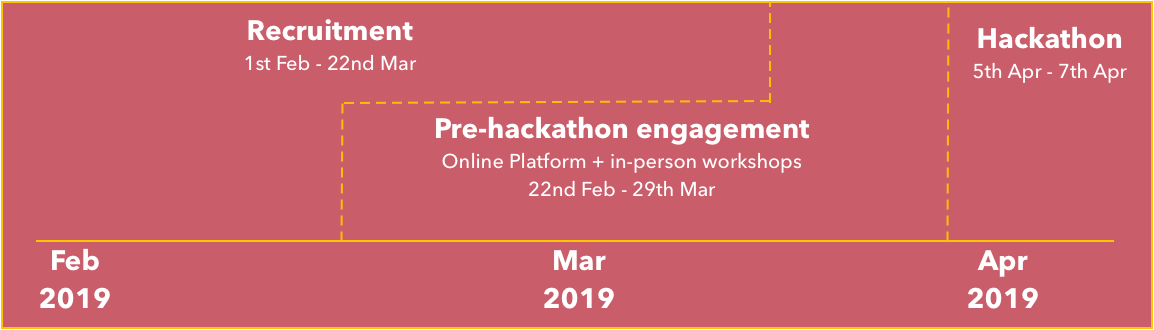
\includegraphics[width=.8\linewidth]{Images/DemVR/Timeline.jpg}
\caption{Timeline of the event}
\label{fig:DemVRTimeline}
\end{figure}

In 2019, I set out to organise a hackathon called DemVR, both to generate a set of bespoke VR environments for those living with dementia, as well as to consider how developers/designers (with expertise in media or VR) and people living with dementia may collaborate. Inspired by prior work involving lived experiences in hackathons \citep{birbeck_self_2017}, the hackathon was split into two engagement phases (see figure \ref{fig:DemVRTimeline}). The first was a six-week pre-hackathon phase: this consisted of the deployment of an online platform (called Ideaboard) to support designers/developers in pitching their potential hackathon ideas and receiving feedback from people with dementia and care partners. The second phase was the two-day hackathon event itself, where participants formed teams to compete for £1000 and £500 prizes by creating prototypes of VR environments for people with dementia and their care partners. To accommodate funding for venue hire, branding, food and travel, I partnered up with several organisations in the city of the university who assisted in the funding and providied expert knowledge on dementia, VR, and running tech-focused events. In the following sub-sections, I describe the event according to the timeline of the hackathon: \ref{sec:EventRecruitment} recruitment; \ref{sec:EventPrehackathon} pre-hackathon - online platform and in-person workshops; \ref{sec:TeamFormation} team formation event; and \ref{sec:HackathonEvent} the two-day hackathon. Additional details of the schedule can be found in the online appendix \ref{app:DemVREvent}.

\subsection{Recruitment}
\label{sec:EventRecruitment}
The initial recruitment process targeted designers and developers through university networks and VR/AR labs across the UK, as well as publishing blog pieces on popular VR websites to invite creators to take part in the two-day event (see appendix \ref{app:Branding} for branding visuals). Upon registering for the event, participants were sent an email inviting them to sign up for Ideaboard and submit their idea. During the recruitment phase, I attempted to recruit people with dementia and their care partners in multiple ways. The first was through a series of invitations across Newcastle that consisted of recruiting through Silverline Memories \added{(similar to chapter four)}, flyers and posters sent out to a range of public spaces that are often used for dementia-friendly meetings and gatherings. Secondly, given Twitter is a popular social media platform for dementia advocates \citep{talbot_how_2020}, I ran a Twitter account posting tweets to encourage people with dementia and their care partners to sign up. I also reached out to several dementia networks such as `World Young Leaders in Dementia' to share the event information on their public newsletter and bulletin boards. 

\added{Due to the addition of the online platform, recruitment altered slightly compared to chapter five, where I was anticipating recruitment across multiple locations and stages of dementia.} In these instances, while I invited people with dementia and care partners to the hackathon, my priority was signing them up to the online platform or to take part in the in-person workshops as the pre-hackathon phase supported longer-term engagement. However, as I have mentioned above, the recruitment processes to involve people with dementia and care partners was challenging, with only one care partner signing up to the online platform.

Twelve participants (two women, ten men) actively signed up to the online platform. During set-up, to initiate conversations, I added three initial example ideas focusing on shared family VR experiences, personalising the VR headset and a VR experience that blends the real world and virtual into one. Out of the 12 participants, eight submitted ideas. Of the 12 participants, nine attended the hackathon (see table \ref{table:DemVRDemographic}), with two submitting an idea but not attending the event. One participant, a care partner named Denis, was unable to attend the hackathon but actively joined discussions on six of the submitted ideas. Additionally, while I set up two in-person workshops (described in section \ref{sec:EventPrehackathon}), the workshops received no sign-ups, resulting in no additional feedback for teams from people with dementia or their care partners. In the discussion, I reflect on why this might have been the case and its implications for public engagement.
For the hackathon, I had 40 participants (18 women, 22 men) in attendance. In the pre-hackathon team formation stage, there was an additional team of four that dropped out due to intellectual property concerns. This resulted in nine teams. Individual demographics of participants within their associated teams are summarised in table \ref{table:DemVRDemographic}. Although no participants had the experience of being a care partner or living with dementia, I defined and solicited participants’ experience with dementia in the following ways:

\begin{itemize}
\item{\textbf{Experienced}: Has worked around dementia in a research/industry/care setting/charity.}
\item{\textbf{Knowledgeable}: Has had a family member or friend living with dementia but not necessarily cared for them.}
\item{\textbf{Limited}: Have read people’s experiences or recent research in dementia.}
\item{\textbf{None}: Know very little about the topic.}
\end{itemize}



\begin{table*}[htp]
% custom commands
\newcolumntype{L}[1]{>{\raggedright\let\newline\\\arraybackslash\hspace{0pt}}p{#1}}
\newcolumntype{C}[1]{>{\centering\let\newline\\\arraybackslash\hspace{0pt}}p{#1}}
\newcolumntype{R}[1]{>{\raggedleft\let\newline\\\arraybackslash\hspace{0pt}}p{#1}}

% this line fixes the vertical padding of text inside the cells
\renewcommand{\arraystretch}{1.4}
\begin{tabularx}{\textwidth}{@{} YYYYYY @{}}
\hline
\textbf{Team} & \textbf{No. members} & \textbf{Age range} & \textbf{Background} & \textbf{Experience with dementia} & \textbf{No. Ideaboard\footnote{members who joined Ideaboard}} \\ \hline 
Garden Life & 7 & 16-25 & Comp-sci undergrads (7) & Limited (1) / None (6) & 3 \\ \hline
Chatter Bench & 2 & 26-45 & History researcher (1) / HCI research developer   (1) & Experienced (1) / Limited (1) & 0 \\ \hline
Augmented World & 6 & 16-25 & Comp-sci undergrads (6) & Limited (2) / None (4) & 1 \\ \hline
VRHallucinate & 6 & 16-35 & Psychology researcher (2) / Developer (3) /   Designers (1) & Limited (1) / None (5) & 0 \\ \hline
LookingVRBack & 4 & 25-45 & Marketing (1) / Biomedical researcher (1) /   Comp-sci undergrad (2) & Experienced (1) / None (3) & 2 \\ \hline
Mindful Forest & 2 & 16-25 & Comp-sci undergrad (2) & Passing (2) & 0 \\ \hline
Sensory Tide & 6 & 26-45 & HCI researcher (3) / Developer (1) / Filmmaker   (2) & Experienced (2) / Passing (1) / None (2) & 3 \\ \hline
World Share & 3 & 16-25 & Filmmaker (3) & Passing (1) / None (2) & 0 \\ \hline
VRmotion & 4 & 16-25 & HCI researcher (1) / Developer (1) / Designer   (2) & Experienced (1) / Limited (1) / None (2) & 0 \\ \hline
\end{tabularx}
\caption{DemVR participant table}
\label{table:DemVRDemographic}
\end{table*}

Expert speakers were also invited to discuss topics on design, dementia advocacy and experiences of living with dementia. An additional three dementia and HCI researchers, a gerontologist and the CEO of Silverline Memories assisted with hackathon facilitation. The facilitators' shared their expertise knowledge by sitting down with individual teams throughout the two days to talk through the teams' ideas and thought processes. The judges consisted of a dementia HCI researcher, the CEO of Silverline Memories, a VR expert and an accessibility HCI researcher to judge the team's final VR ideas.

\pagebreak
\subsection{Pre-hackathon engagement}
\label{sec:EventPrehackathon}
I planned and arranged a six-week consultation period, to be conducted via 1) an online participatory platform, and 2) in-person workshops with people with dementia and their care partners. Additionally, I provided a team formation day prior to the two-day hackathon to allow people to socialise with other participants and form teams if they had not already done so. The pre-hackathon stage provided the optional opportunity for future hackathon participants to submit initial thoughts and ideas where experts would provide feedback to give participants insight into the needs, desires and experiences of people with dementia and their care partners. 

\subsubsection{Online platform (Ideaboard)}
\label{sec:Ideaboard}

\begin{figure}[htp]
\centering
\begin{subfigure}{.5\textwidth}
  \centering
  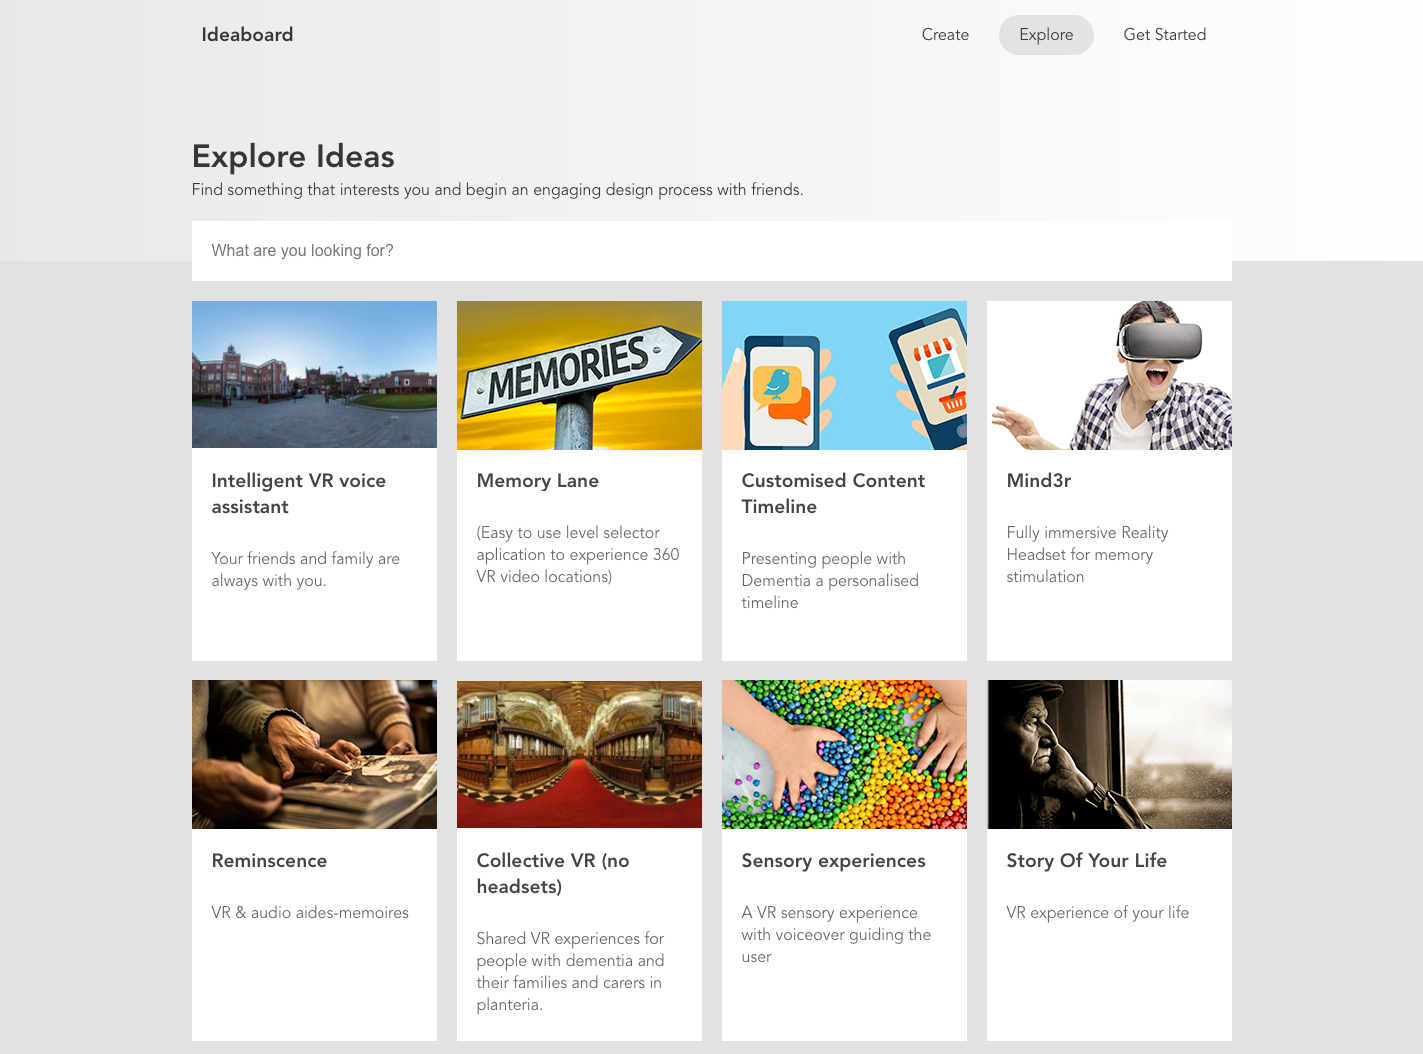
\includegraphics[width=.8\linewidth]{Images/DemVR/Ideaboard Ideas.png}
  \caption{Explore Ideaboard ideas}
  \label{fig:exploreIdeaboard}
\end{subfigure}%
\begin{subfigure}{.5\textwidth}
  \centering
  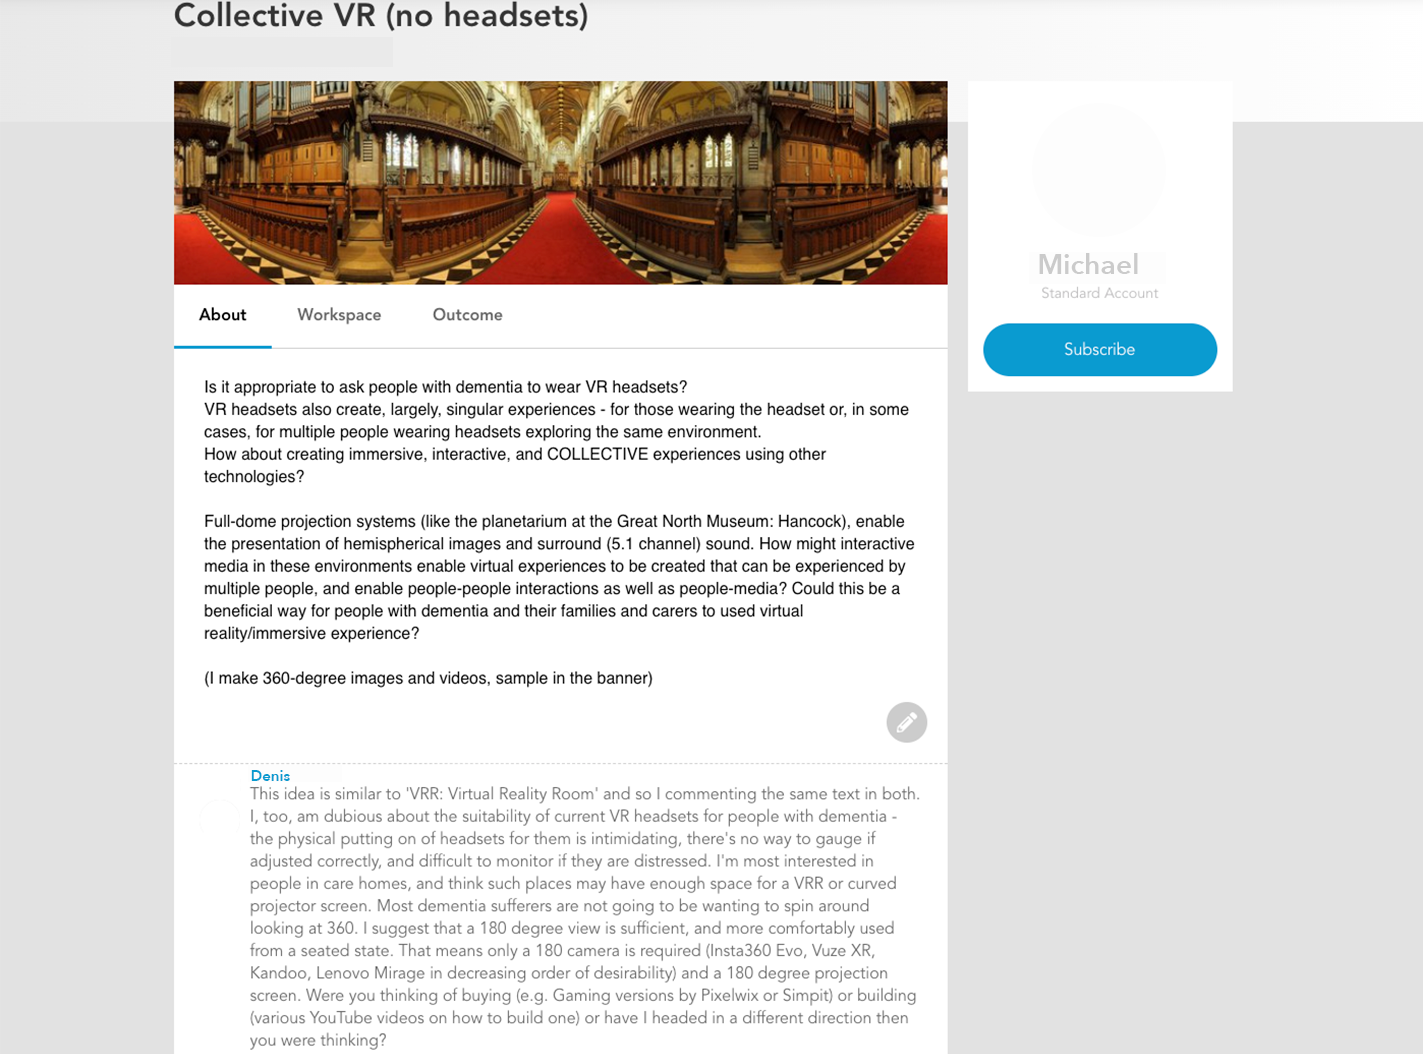
\includegraphics[width=.8\linewidth]{Images/DemVR/Example of idea.png}
  \caption{Example of 'idea' features}
  \label{fig:IdeaboardIdea}
\end{subfigure}
\caption{Ideaboard features}
\label{fig:IdeaboardFeatures}
\end{figure}

The participatory platform, Ideaboard (see figure \ref{fig:IdeaboardFeatures}), was conceptually inspired by participatory platforms such as Kickstarter, GoFundMe and Indiegogo. The platform also takes influence from work in digital civics and social care – for instance, one inspiration was App Movement \citep{garbett_app_2016}, a platform that enables users to \textit{``collaborate, design, and deploy community commissioned mobile applications''}. Ideaboard similarly offers creative tools and workspaces to support the creation of ideas and collaboration. Here, I describe the process users undertake to add ideas to the platform. The Ideaboard process was split into three components:

\begin{enumerate}
    \item On Ideaboard, participants were invited to share preliminary ideas that they could develop during the in-person hackathon. The idea consists of the title, summary of the idea, a detailed description and an optional sketch/mock-up. Once their idea was uploaded, participants could then explore and comment on other submitted ideas  (see figure \ref{fig:exploreIdeaboard}).
    
    \item Once participants had submitted their ideas, I invited people with dementia and their care partners to share insights on and critique the submitted ideas on Ideaboard. I hoped that this would allow people who might be unavailable for the hackathon to take part in design ideation and help to shape emerging ideas that might be taken further in the two-day hackathon. 
    
    \item Hackathon participants could then respond to the expert feedback and begin an open dialogue with other participants, care partners and people with dementia. From here, ideally, teams would have more in-depth and developed ideas that considered the experiences of care partners and/or people with dementia. 
\end{enumerate}

\subsubsection{In-person workshops}
\label{sec:in-personWorkshops}
To further support participation beyond the online platform \citep{piper2016technological}, I set up two in-person workshop sessions inviting members from Silverline Memories. Working closely with the dementia café seen in chapter four, I expected to recruit several people with dementia and care partners with established experience of VR. Within the six-week consultation period, the two in-person workshops were organised in the final two weeks to ensure that I could print off any submitted Ideaboard ideas to share with participants.  This workshop was intended to support participants to engage in a set of design activities to illustrate their desired VR shared experiences or build upon the existing 11 ideas posted on Ideaboard. Based on comments and ideas produced in these workshops by care partners and people with dementia, I would then add any additional ideas to Ideaboard or add any comments made about existing ideas to the relevant Ideaboard idea. I hoped that this process would allow the designers/developers to have additional time to reflect on comments from people with dementia and their care partners. As stated in the recruitment, the attempts to involve people with dementia and their care partners was significantly limited to one care partner’s involvement which engaged through the online platform. For both in-person workshops, I received no sign-ups, meaning that I had to cancel the workshops. I refer to this in more detail through the findings and discussion.

\subsection{Team formation}
\label{sec:TeamFormation}
I set up a two-hour pre-hackathon team formation event on the Friday of the hackathon weekend to ensure that participants had organised themselves into teams. During the team formation event, I printed the 11 ideas published on Ideaboard. I placed them on individual tables where participants could add a sticky note to express an interest in the idea. Since submitting an idea on Ideaboard was optional, five teams came prepared with ideas. As a result, only four of the 11 Ideaboard posts were taken into the hackathon. In the online appendix \ref{sec:EventIdeas}, I present the origin points of teams’ initial ideas. During the hackathon, all teams adapted their original ideas by reflecting on how people with dementia might experience them. They did this through engaging with a series of resources (discussed below), and otherwise used the time to build and design a rudimentary prototype of their VR experience. 

\subsection{Hackathon}
\label{sec:HackathonEvent}
\begin{figure}[htp]
\centering
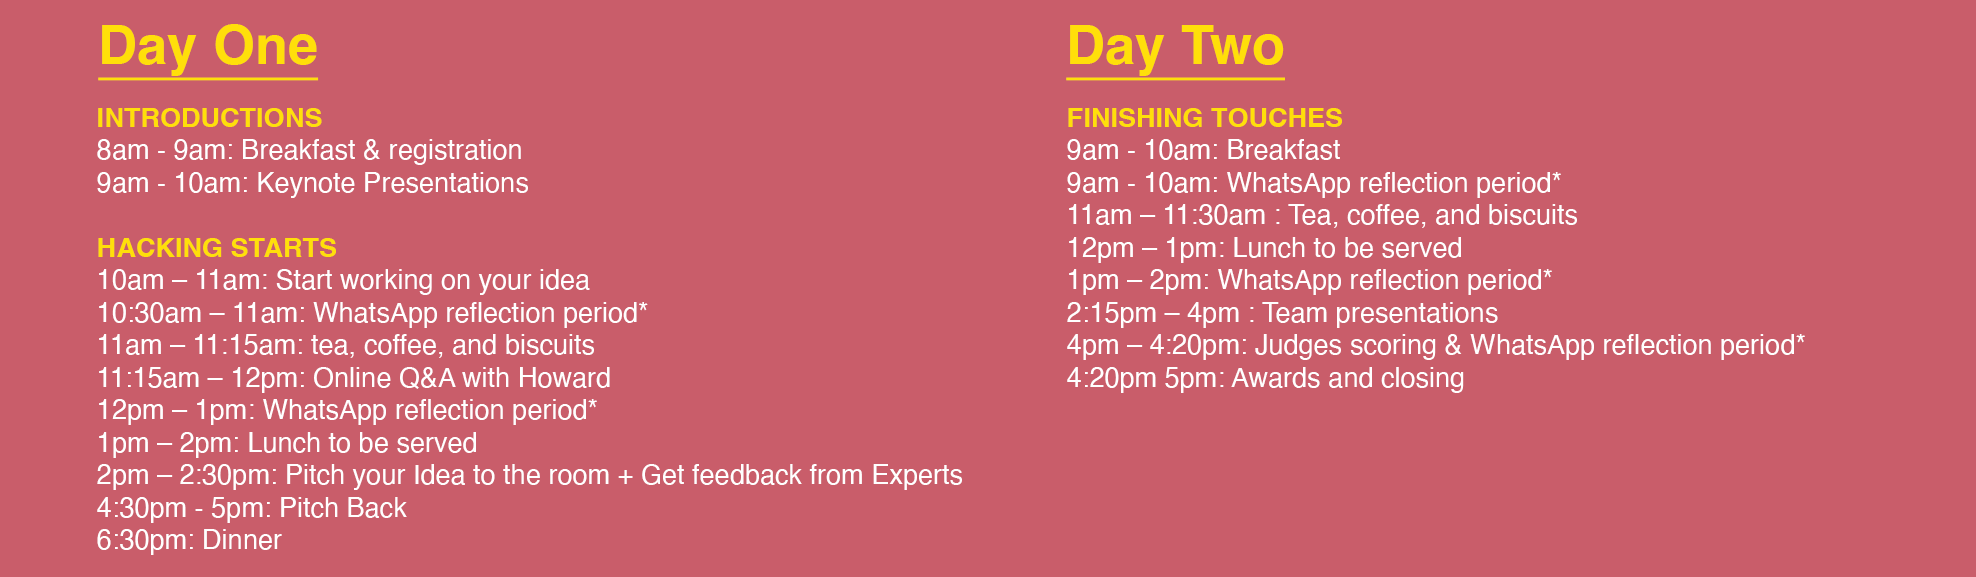
\includegraphics[width=1\linewidth]{Images/DemVR/DemVRHackathonSchedule.png}
\caption{DemVR hackathon event schedule}
\label{fig:schedule}
\end{figure}
The hackathon took place across one weekend (April 5\textsuperscript{th}-7\textsuperscript{th} 2019), at a local museum in Newcastle. The venue situated within the city centre near the university campus and co-exists alongside a Natural History Museum to which attendees had access to throughout the two days, which provided space away from `hacking'. To accompany the large number of teams and space required for VR demos, each team received a demo space, rounded table and an array of crafting materials. For additional details of the schedule, please see appendix \ref{app:DemVR:EventSchedule}. In terms of equipment, teams had access to eight Oculus Go’s, four Oculus Rifts, one HTC Vive and two VR-ready PC rigs. Teams were encouraged to bring their laptops and VR kit if they wished, and to notify the facilitators before the event if they needed any additional technologies.

\subsubsection{Day one}
\label{DayOne}

\begin{figure}[htp]
\centering
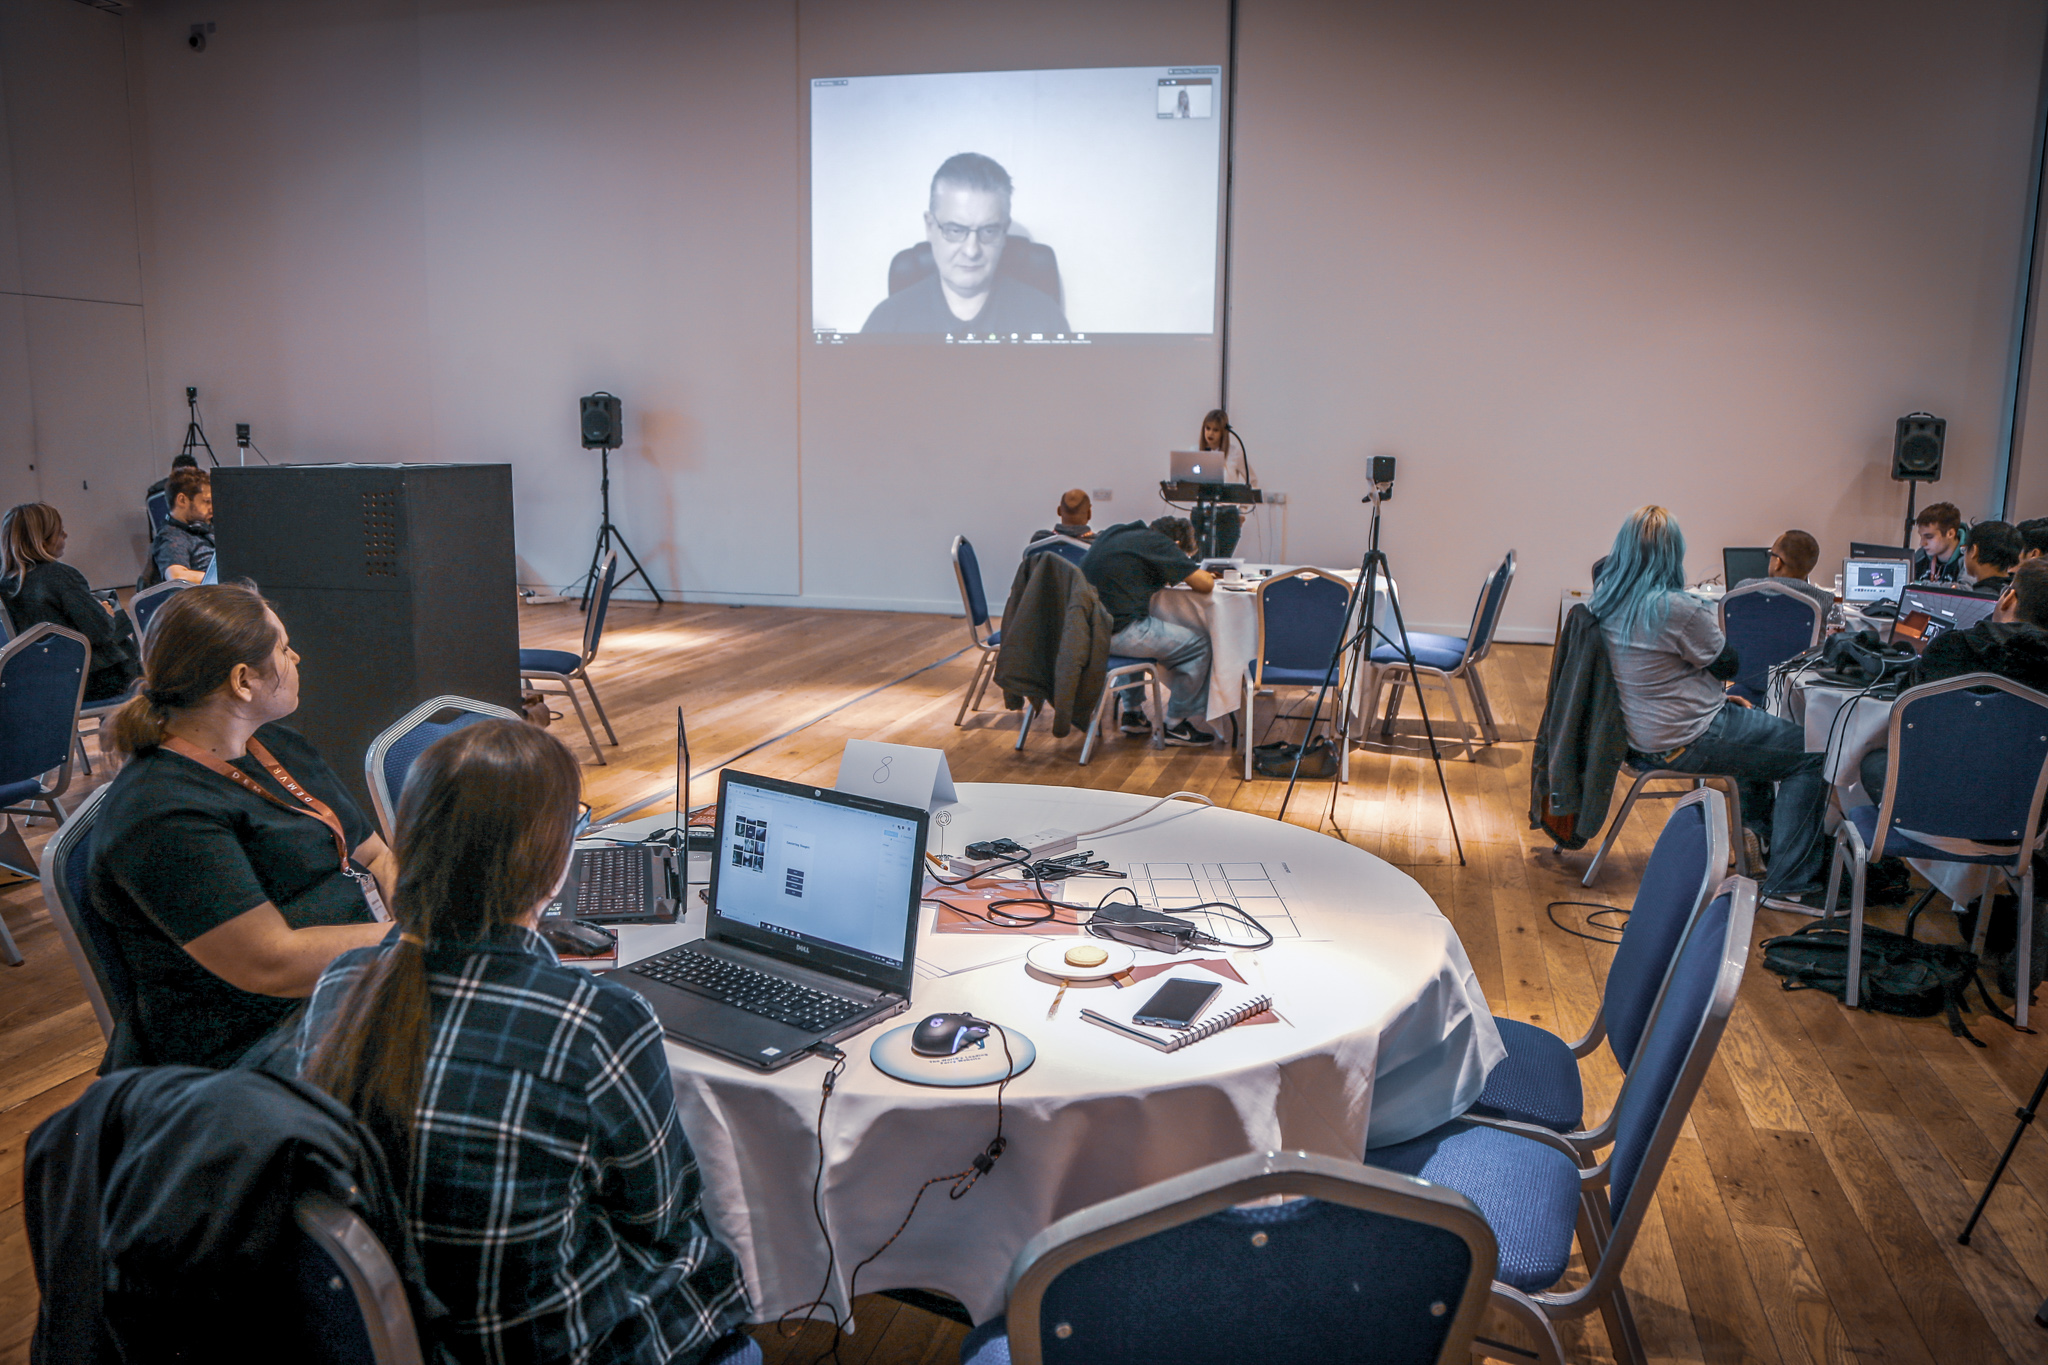
\includegraphics[width=.4\linewidth]{Images/DemVR/Howard.jpg}
\caption{Howard's Zoom Q\&A}
\label{fig:Howard}
\end{figure}
The first morning of the event consisted of presentations on dementia, participatory research and VR by invited speakers. The invited speakers also acted as facilitators who provided hackathon participants with insight into their backgrounds. Over the mid-day period, I organised an online Q\&A with Howard, a dementia advocate who shared his experiences living with dementia, which lasted 15 minutes. In the Q\&A, Howard was asked about his challenges of being diagnosed, the types of technologies and experiences he would find useful, and the social complexities he is currently facing given the stigma of dementia. While the Q\&A was open for questions from the participants, the conversation was led by one of the keynote facilitators who had a strong relationship with Howard (see figure \ref{fig:Howard}).

After this, teams began to `hack'. Teams could then ask for additional help or critique from facilitators, either in person or reaching out to them in the individually set up WhatsApp team groups. In practice, these online chats with facilitators provided quick and easy links to papers or method approaches that were related to the topic at hand. Furthermore, I used these groups chats as an opportunity to a) ask participants to respond to reflective questions such as \textit{``How have your thoughts about dementia and/or virtual reality changed from the beginning of day one?''} and \textit{``Describe your reaction to Howard’s Q\&A''}, and b) invited them to detail their project’s progression through submitting comments, audio recordings and videos through a dedicated team WhatsApp group chat, which formed the basis of data collected during the event. For instance, team Sensory Tide shared pictures of team members travelling to a local beach to collect videos and shells to be used in their finalised idea.

Teams were given inspiration packs (see figure \ref{fig:InspirationPacks}): these consisted of materials that summarised key insights from the previous work I did on dementia and VR (the two studies from chapter four). In addition to the physical inspiration packs, I set up an online shared document that would continue to grow as a resource through the duration of the event. In the end, this consisted of academic papers; speaker slides; dementia guides such as DEEP language and NHS (UK National Health Service) guides; a set of handouts detailing design processes such as scenarios, bodystorming, and 5 Whys; and tips and tricks for what to include in the final presentations. In the findings, the DEEP language guide is drawn upon several times; it is a three-page document designed by 20 people living with dementia \citep{diaries_deep_2020}. The key takeaways of the document are a set of standards for accepted or sensitive ways to talk about dementia. During the afternoon, all teams pitched their idea to the rest of the room. This provided an open forum between facilitators and participants to provide additional feedback for the set of ideas. For the rest of the weekend, the teams worked on their ideas with periods built in for breaks and socialisation. 

\begin{figure}
\centering
\begin{subfigure}{.5\textwidth}
  \centering
  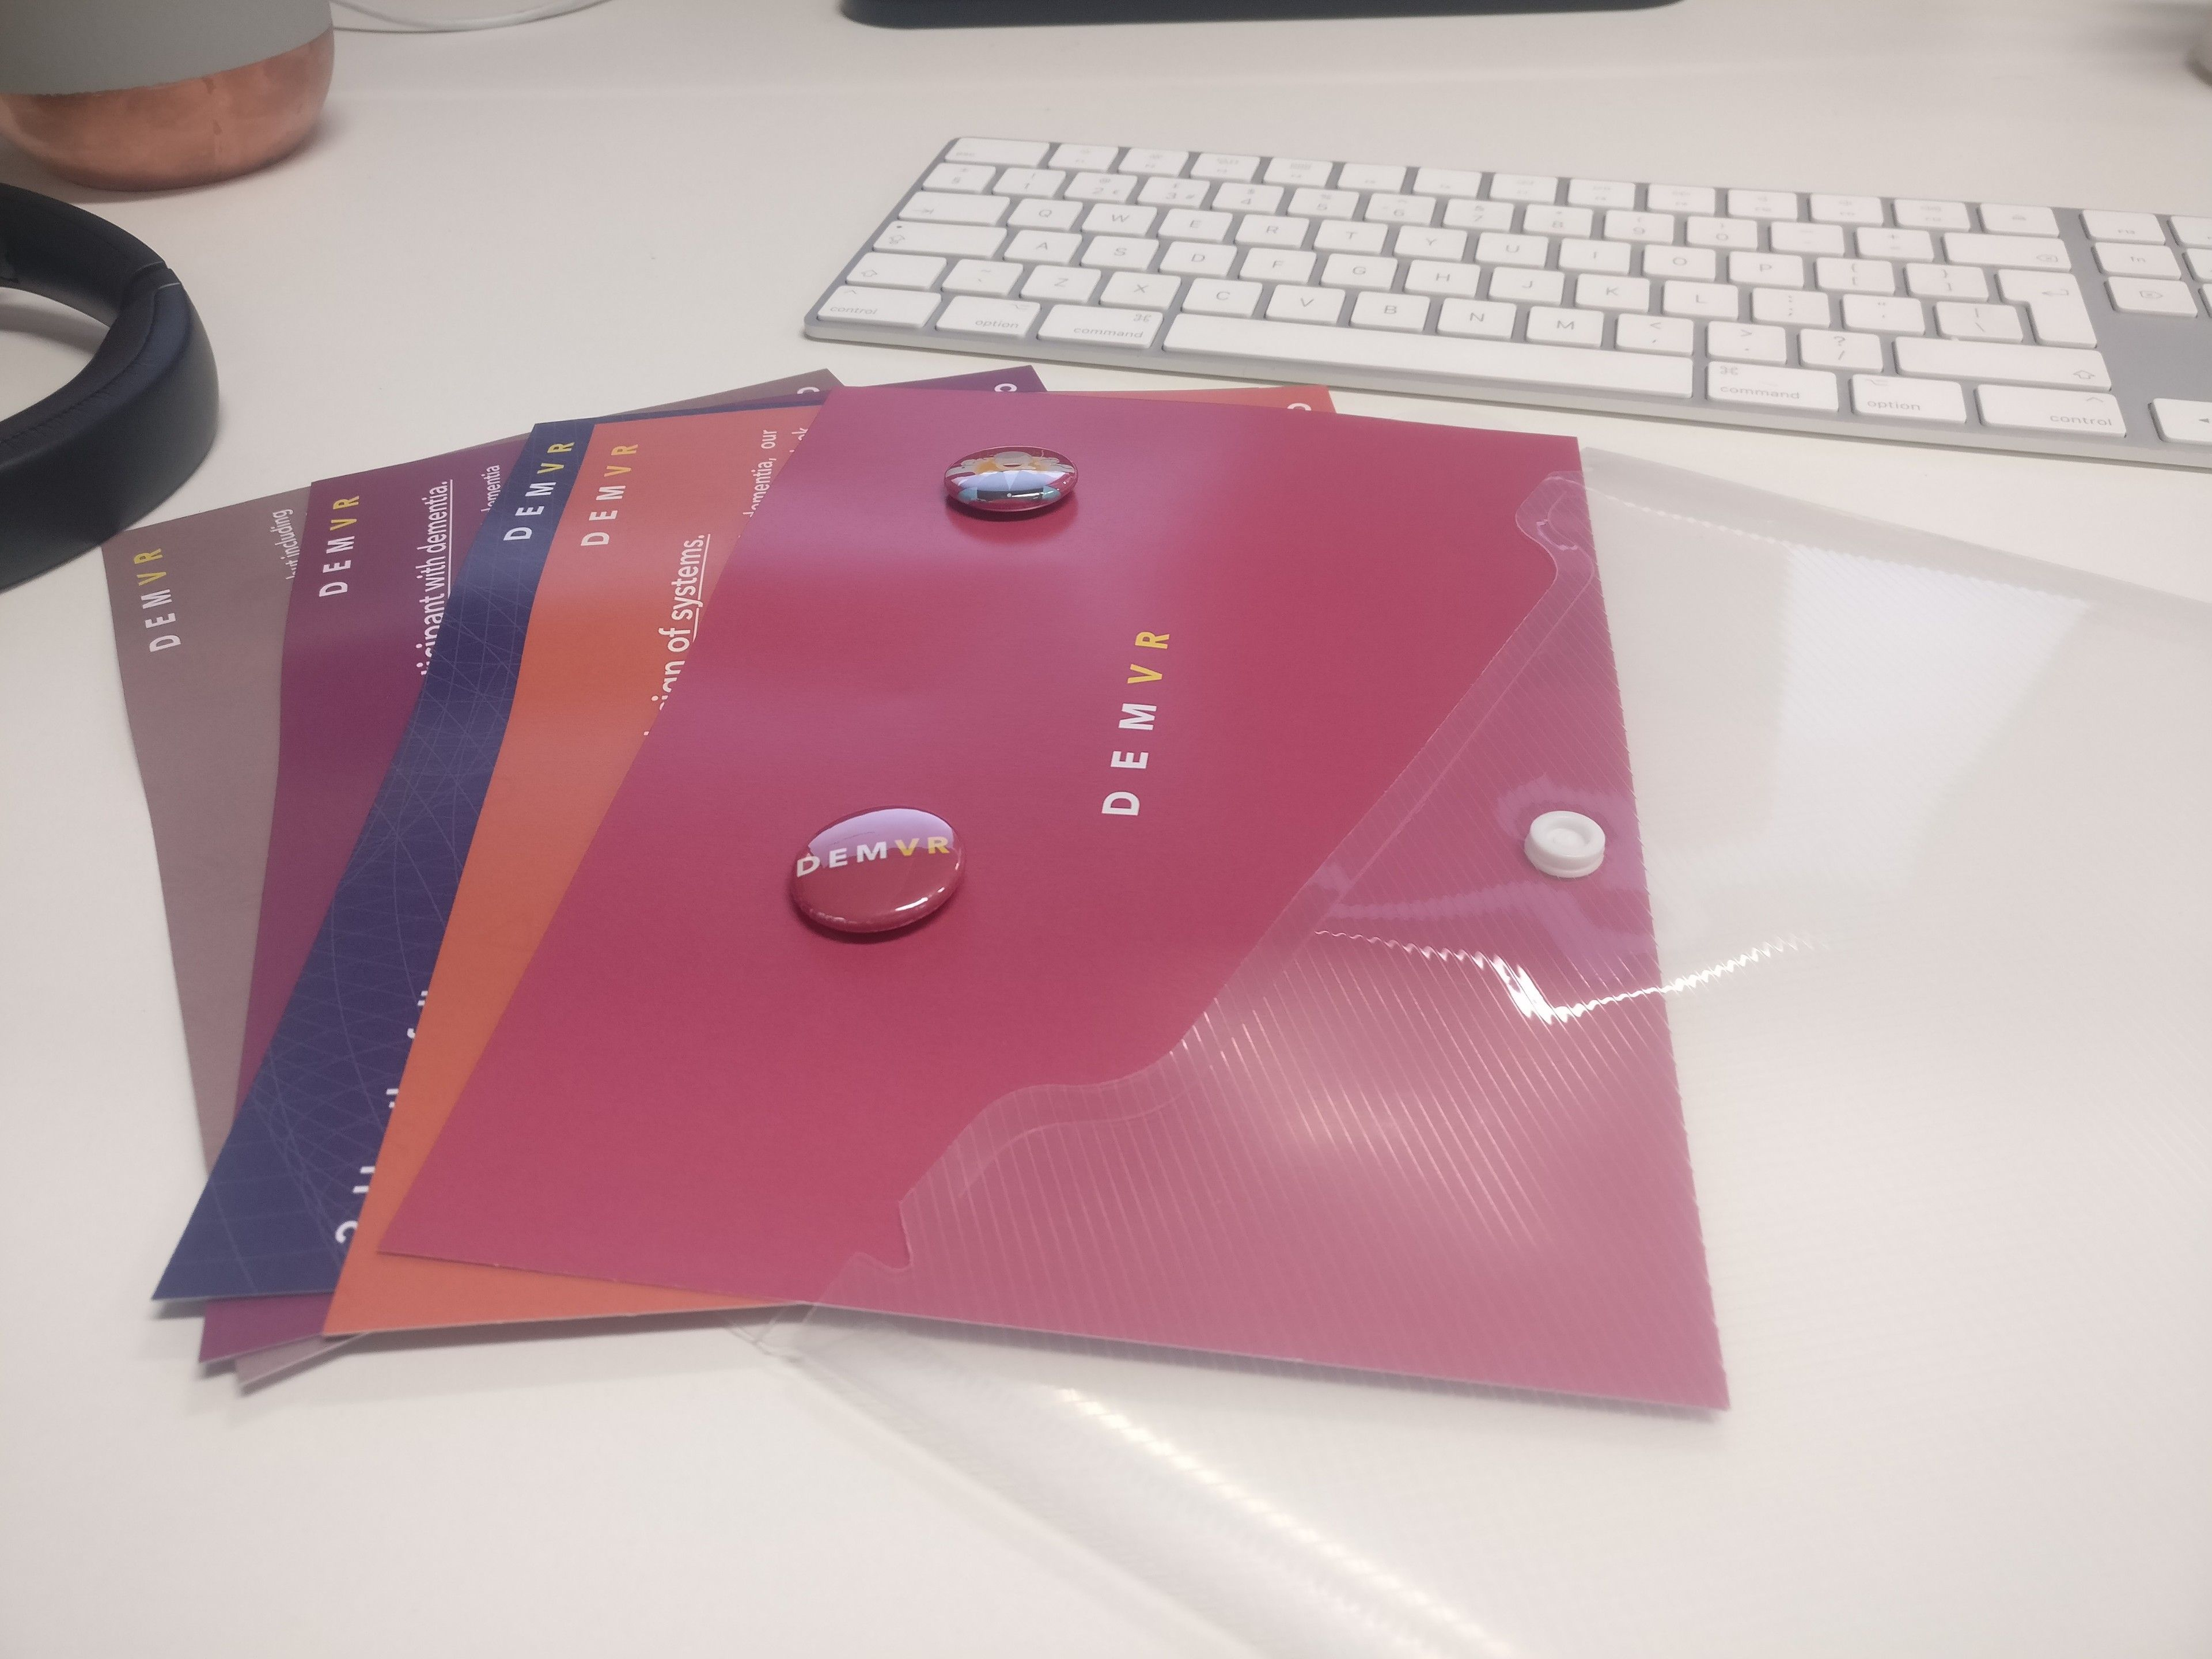
\includegraphics[width=.8\linewidth]{Images/DemVR/DemVRInspiration.jpeg}
  \label{fig:InspirationPackImage}
\end{subfigure}%
\begin{subfigure}{.5\textwidth}
  \centering
  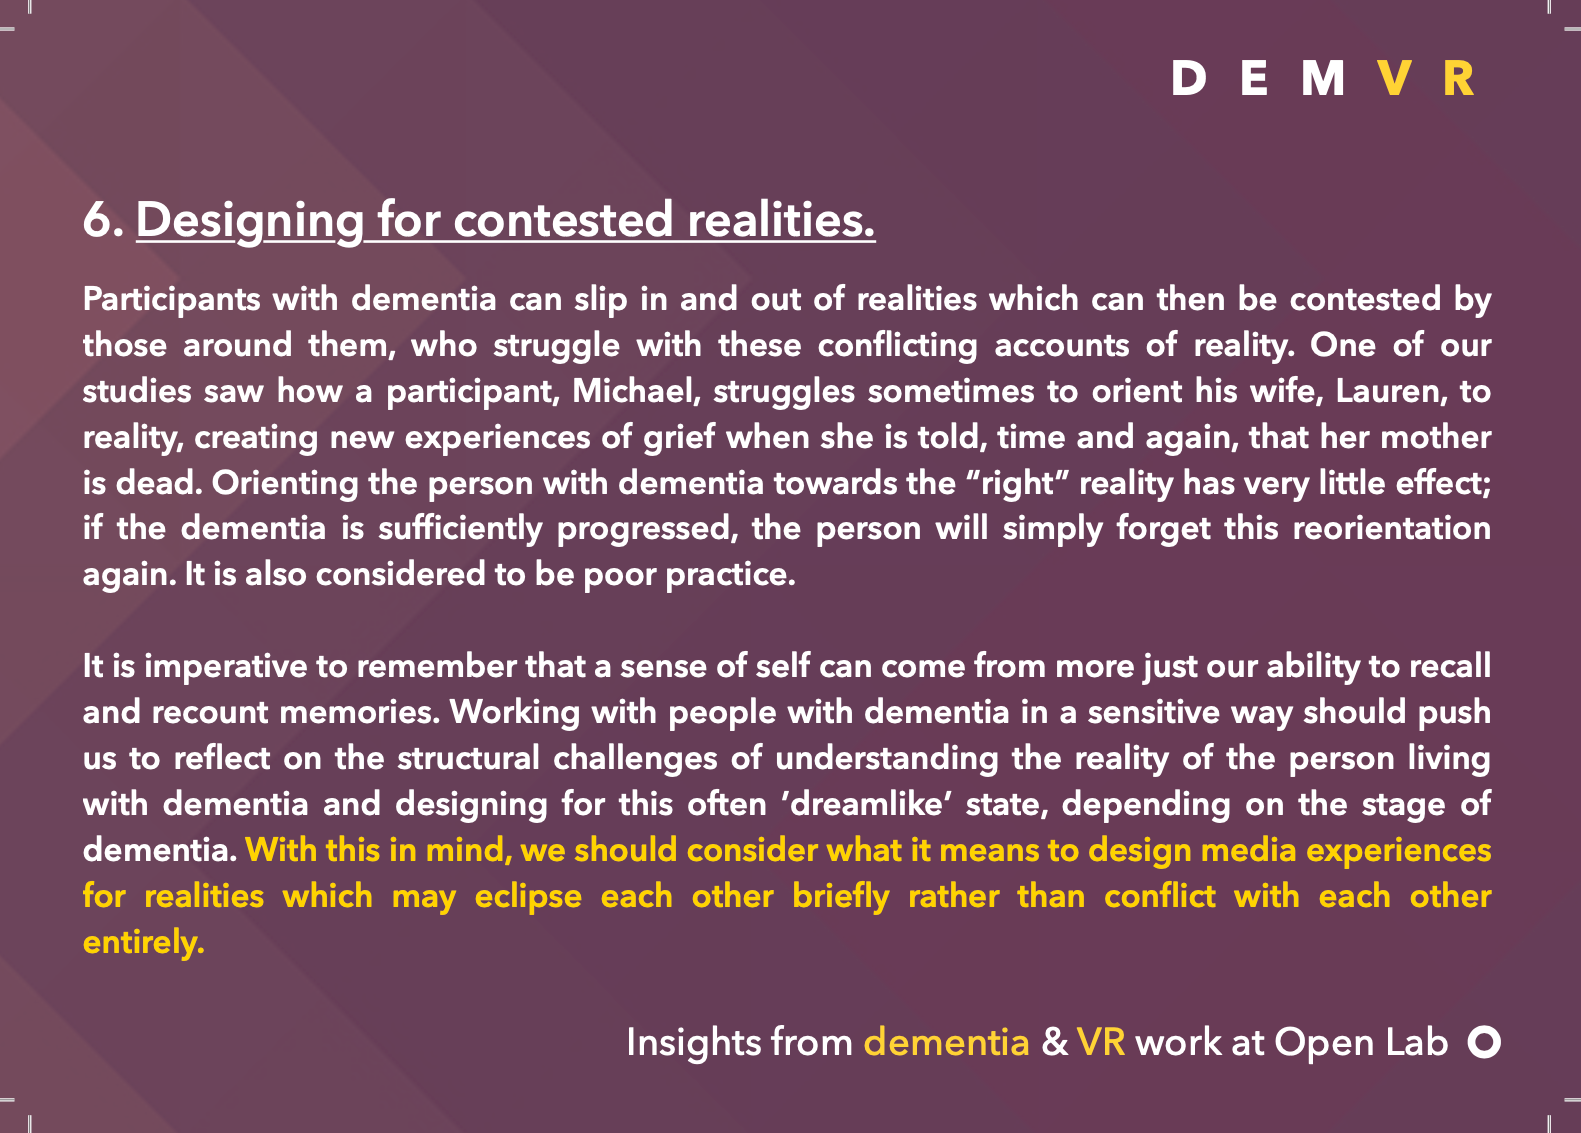
\includegraphics[width=.8\linewidth]{Images/DemVR/InspirationCard.png}
  \label{fig:InspirationCard}
\end{subfigure}
\caption{Inspiration packs}
\label{fig:InspirationPacks}
\end{figure}

\subsubsection{Day two}
\label{DayTwo}
On the Sunday morning, teams had the entirety of the day to finalise their ideas and presentations and had the opportunity to ask facilitators for feedback on their presentations and demos. Facilitators assisted in helping teams add finishing touches to their demos and provided feedback on their presentations. To maintain consistency, I provided a template with guiding topics such as: title and tagline; who is your user audience; what is your motivation and problem; what was your approach to inform your design challenge; what are the future considerations; and reflection on the hackathon. The event culminated in each team presenting a final ten-minute presentation and five-minute demo that allowed teams to demonstrate their work to the judges. The four judges had the opportunity to explore the demo and ask any further questions about the teams' finalised ideas. Each team’s finalised concepts were rated on the following:

\begin{itemize}
\item Novelty of design concept: How original are the ideas? Are they backed up with appropriate research? How provocative (yet sensitive) or otherwise promising are they?
\item Clarity of team's vision: How persuasive are the presented arguments?
\item Sensitivity to the challenge: Specificity to issues central to dementia/care; How well were experts’ suggestions taken on board? Are there any potential negative consequences?
\item Potential for real-world impact: Given appropriate backing or resource, would this concept make a difference?
\item Strength of VR/AR: How far along did the idea development get? Did the teams make good use of the technology at hand? 
\end{itemize}

At the end of the day, the judges announced the first and second place winners who would receive £1000 and £500, and the event ended with a brief overview of the hackathon. Teams' proposed ideas can be found in the online appendix \ref{sec:EventIdeas}.

\section{Methodology}
\label{sec:methodology}
Following the event, I began to reflect on how the event unfolded and the study's potential contribution to HCI research. Although the initial focus of the event was on bridging the gap between the designers/developers and the topic of dementia, given the challenges I faced in representing people with dementia and their care partners, I saw this as an opportunity to provide guidance for future researchers on the potential knock-on effects when designing for a user group who are missing from the design process. To guide my analysis with relevant research questions, 

\begin{itemize}
    \item \textbf{Research Question One:} How do designers/developers represent people with dementia when solely relying on their own experience (or lack thereof)? 

    \item \textbf{Research Question Two:} What considerations for technology do designers/developers prioritise when designing for people with dementia?

    \item \textbf{Research Question Three:}  What challenges arose when trying to represent the voices of people with dementia and care partners during the hackathon? What opportunities arose that we may, in time, pursue?
\end{itemize}

\added{With these three RQs, they are an extension of the thesis research questions in order to maintain a focus throughout the chapters analysis. In the chapters summary, I return to the original research questions and map them to relevant insights found in the chapter.}
\subsection{Ethics}
\label{sec:Ethics}
Ethical approval was granted by Newcastle University. Upon signing up, each participant was provided with an information and consent form describing the event and pre-hackathon stage. Any participants who then signed up to use the online platform were given additional information about the project. Participants who registered for the hackathon signed a consent form about the hackathon weekend when they came to pick up their lanyard and sign in for the opening day of the hackathon. Participants’ and teams' names have been anonymised for privacy.

\subsection{Data and analysis}
\label{sec:DataAnalysis}
In the study, I gathered data from four different sources: 1) the text data of the Ideaboard ideas (I), including additional comments from participants on the ideas; 2) the keynote, Q\&A and teams’ presentations from the event (P); 3) each team’s WhatsApp group’s texts (W), images and audio, which were extracted using the built-in Google Drive feature; and 4) my observational field notes (F) taken throughout the event highlighting conversations they had with teams and facilitators. Audio recordings collected through WhatsApp were in response to five questions asked over the weekend that I described above. WhatsApp audio recordings were also transcribed and anonymised by UKTranscription. The initials (I, P, W, or F) indicate the source of the data in the findings.

\begin{table*}[ht]
\begin{tabularx}{\textwidth}{@{} Y|YYYYY @{}}
\textbf{Stakeholders} & \textbf{Ideaboard (I)} & \textbf{WhatsApp (W)} & \textbf{Presentations (P)} & \textbf{Field notes (F)} \\ \hline
Hackathon participants & 11 submitted ideas & 25 minutes audio recordings + average 25 texts per team & 117 minutes & N/A \\
People with dementia and care partners & One care partner replied to 8 submitted ideas & N/A & 15 minutes Q\&A & N/A \\
Facilitators & N/A & Average 6 texts replying to each team & 40 minutes & 11,355 words \\
\end{tabularx}
\caption{Data collection}
\label{table:data collection}
\end{table*}


My analytic approach followed a Thematic Analysis (TA) set out by \cite{braun_one_2020,braun_using_2006}. \added{In contrast to the studies presented in chapter four,} to make sense of interactions between data sets, I used the recorded keynotes, Q\&A and team presentations to structure an organised timeline of the individual sets of data. This approach helped to decide if it was possible that a certain event, such as a keynote or the Q\&A, had influenced a team's design approach, though the qualitative approach is careful in not claiming causality. Second, I structured a set of team narratives consisting of the different data sources described above. Structuring the data in this way helped to describe the chronological development of each individual team from design ideation through to presenting their final idea and post-hackathon reflections.  Once the data was framed chronologically, I began to conduct open coding. I then worked with Dr Kellie Morrissey, Dr Sarah Foley and Dr Dave Kirk in bi-weekly meetings to construct themes and reflect on the patterns evident across the data. Finally, I constructed the named themes, which are presented in the next main section. 

\section{Findings}
\label{sec:Findings}
The findings comprise of three themes, which have been identified through a semantic approach to analysing the data corpus. The first theme details participants’ motivations for participating in the event. The second theme provides insights into participants' challenges and design techniques, given the absence of crucial stakeholders. Finally, the third theme unpacks the teams’ final prototypes to explore their new understandings and considerations for dementia within their design.

\subsection{Motivations behind participation}
\label{ThemeOne:subthemeOne}
Participants’ motivations for taking part in the event ranged from their own personal experiences of loved ones with dementia, seeking a chance to win the cash prize, sharing their voice, and learning about the area of dementia and HCI. This speaks to the varied emotional and technical entry points for the participants. For those with personal experiences, the concerns and needs of family members were central to the teams’ ideas. For instance, in team World Share’s presentation, one member, Michael, described conversations with their grandmother with his grandfather where \textit{``he may not remember going to the beach that day but he’s happy, and it’s about the day-to-day quality of life, which is something we’re looking to do with [our idea]''} (P). \added{Similarly to those studies presented in chapter four,} David from Chatter Bench, described family connections influencing their involvement where they \textit{``called [his] mum [to talk about his] grandparents who were living with dementia in a home before they died … this informed what was important [to them joining the event]''} (P). \added{The drawing on family history and experience resonated with my own motivation seen in chapter four, with designs informed by the context of a specfic user and their needs.}

For others who had research experience in the field, their reasoning for taking part was rooted in learning how VR could be a beneficial technology within this space. For instance, one member from VR Motion was working on \textit{``intergenerational interactions in dementia care''} (P) and came to the event to \textit{``learn how VR and dementia can be linked together''} (W). Undergraduate teams echoed similar comments where VR Hallucinate could learn about \textit{``how technology can help dementia''} (W), or Garden Life asking, \textit{``What can I do to help people with dementia?''} (F). In this sense, the teams are seeking out a technical and social knowledge to inform design of appropriate technologies in their work. At the end of Garden Life’s presentation, they expressed that \textit{``events such as [this hackathon], continue to be run to deepen our understanding of such issues [to] help alleviate the stigma that caused [negative representations] to happen''} (P). This demonstrates the team’s reflections on the value in the learning process through the hackathon. Perhaps unsurprisingly, a sense of competition and prize money were significant motivators for several teams. My field notes described \textit{``how [teams] would come up to the [primary facilitator] and say they’re going to win the prize money as their idea is the best''} (F). While this made for particularly enthusiastic participants, in many ways, it could also be seen to hinder collaboration between teams. Moreover, it was also a potential contributor as to why there was little uptake from the participants in using the online platform, which would have made participants’ budding ideas public knowledge.

\begin{figure}[htp]
\centering
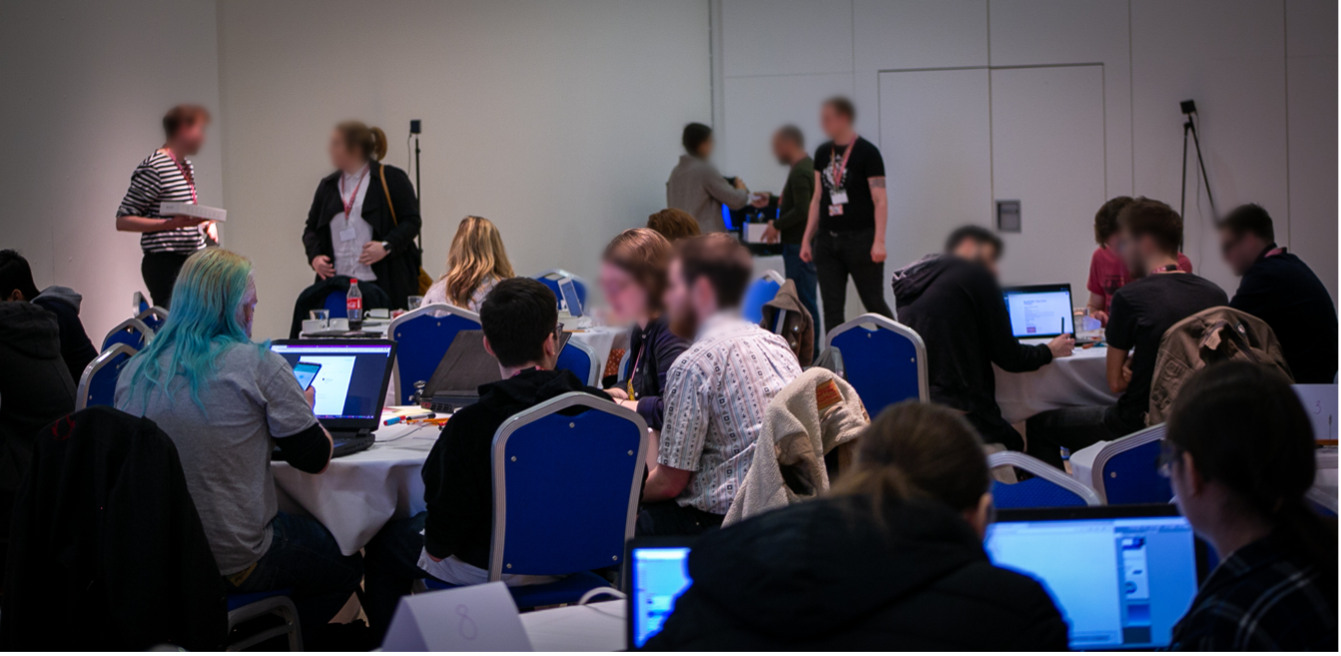
\includegraphics[width=.8\linewidth]{Images/DemVR/Findings/DayOneDemVR.png}
\caption{Day one of DemVR}
\label{fig:DayOne}
\end{figure}

For others, their motivation to take part clashed with the event's goals. For example, a team of VR developers from a game company, dropped out during team formation with concerns about revealing their idea to the extent of questioning \textit{``who owns the intellectual property''} (F) of the idea. During the pre-engagement phase, I made it clear to the teams that the university would not progress or develop any idea, I simply wished to potentially describe their ideas in academic work. However, the team remained hesitant to continue as \textit{``people could read the paper and steal the ideas and build it themselves''} (F).  Additionally, Rachel from Sensory Tides raised a similar concern with publication as they wanted to \textit{``build [their] idea into an academic paper''} but felt wary that the \textit{``novelty of the idea may have worn off once the event had published the idea''} (F). While only one team left, motivation to collaborate or share ideas that could be fleshed out into a commercial product remained relatively scarce between those with expertise in and knowledge of VR or dementia research. 

As described in the event context, there was little motivation to participate in the pre-engagement phase. From the 12 participants in this phase, Denis was the only care partner who signed up and participated with the other designers/developers. Denis was motivated to share his experiences of his father’s dementia, hoping outputs of the event would provide \textit{``published prototypes [he] can use [with his father]''} (I). As Denis continued to comment on the Ideaboard ideas, he would identify limitations in people’s ideas, saying: \textit{``my father is too old to use social media''} (I), or \textit{``my father wouldn’t understand how to navigate in VR''} (I). In these examples, Denis was advocating on his father's behalf to make sure his father’s challenges were considered in future VR outputs. Although Denis expressed his motivation in the development of VR technologies for people with dementia, the planned in-person workshops with people with dementia raised concerns about interest when \textit{``no-one signed up to the workshops ... CEO of the café just notified me and asked if we should cancel the [the workshops]''} (F). From the my field notes, at the time, I felt \textit{``perhaps members [of the café] are no longer interested in VR work anymore''} (F). \added{Likewise, when I reached out to recruit families with dementia who I involved in chapter four, the families themselves expressed a lack of interest in taking part in more VR research as they felt it} \textit{``was too complicated''} for them after having spent significant time using an Oculus Go headset. \added{Furthermore, families motivation to participate in the study in chapter four were primarily due to the days out and building of the moments boxes. While they were also uninterested in the hackathon structure, they still expressed interest in going on} \textit{another day out''} that would be similar to previous study. 

From this theme, it is evident that there were intersecting, and sometimes opposing, motivations for taking part in the hackathon, ranging from personal experience, competition or opportunities to upskill and expand their research/development profile. This diverse range of motivators has implications for event organisers, who may need to consider how the event can attend to emotional, social and technical support required of the teams. Pre-engagement may be an important time to ask teams to reflect on their motivations for taking part and pre-empt any support needed. 


\subsection{Constructing the absent user}
\label{ThemeTwo:AbsentUser}
In response to the `absent user', ideas were generated and developed over the course of the event through interactions with facilitators, inspiration packs and Howard’s Q\&A. I noted that participants often focused on comments made by speakers who discussed their experiences with people with dementia. For instance, during World Share’s presentation, Michael described learning from \textit{``some of the expert [facilitators], that dementia is more than focusing on memory loss''} and instead their idea focused on \textit{``designing experiences that are set in the present, inclusive, and can be shared with others that are going to make a connection''} (W). This demonstrates the team’s willingness to learn about dementia and incorporate feedback into their design ideas.

The interplay between the stories, resources and conversations scaffolding the event helped to create an initial understanding of what it might be like to live with, and design for, dementia. Due to the lack of people with dementia and care partners involved in the event, several teams drew on Howard’s experiences of dementia that he shared in his 15-minute Q\&A to understand the potential challenges and opportunities he may want in a VR environment. \added{In contrast, in chapter four, I was able to iterate and design with a variety of experiences of dementia from not only the person with dementia, but also family member perspectives too}. For those teams, Howard became a pivotal resource, and a somewhat static personality they were designing `for'. The ways in which teams reacted to Howard’s experiences varied. Team Garden Life changed their design approach in response to Howard's hobbies and interests: their initial idea centred around \textit{``a journey through the story of your life using different media that links memories with locations' ''}. (I) They stated that \textit{``The experience can be customised by family, so that the focus is on either neurological rehabilitation or reminiscence''} (I). In response to Howard’s Q\&A, the team developed a VR `garden', with a feature that allowed the user to interact with a virtual dog. In the WhatsApp group chat, the team state that they \textit{``found it interesting [that Howard] has a pet dog''} (W). This led to the team reflecting on how people living in a care home may not have that opportunity, but that \textit{``having an animal to care for seems to help people in a lot of ways''} (W); and the team felt a virtual dog could help with loneliness (seen in figure \ref{fig:GardenLifeDog}). Translating Howard's experience into features for their design helped the teams to incorporate aspects of Howard's lived experience into their design, rather than focusing on dementia and its related symptoms. 

\begin{figure}[htp]
\centering
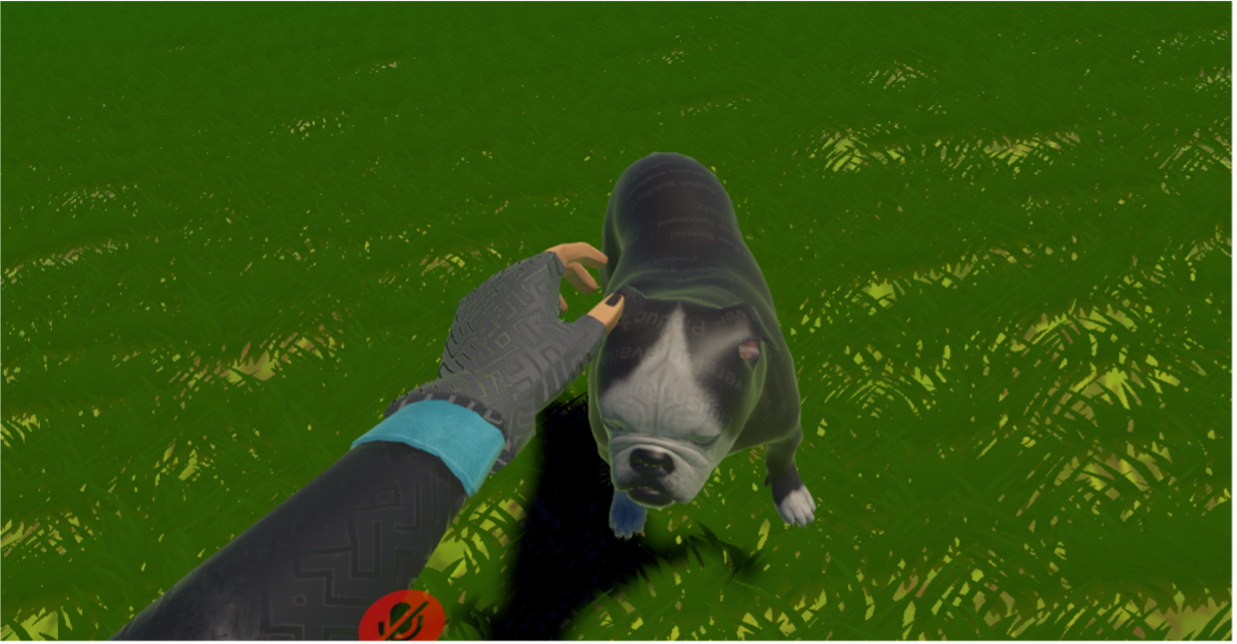
\includegraphics[width=.8\linewidth]{Images/DemVR/Findings/GadenLifeVR.png}
\caption{Garden Life's VR dog companion}
\label{fig:GardenLifeDog}
\end{figure}

As the team developed the garden environment further, they built customisability options: \textit{``you can change its breed, colour and name of the animal''} (W). Similarly, for Mindful Forest, Howard’s experiences provided an opportunity to expand their current understandings of dementia as they \textit{``realised [they] actually don’t know as much [about dementia]''} (W). In response, the team’s final idea featured \textit{``family members adding various pictures from holidays when they were young, so it would help in remembering if they forgot about their grandson or grand-daughter''} (P). While the team prioritised their experiences of dementia where \textit{``I still remember the day when my grandma no longer recognised me''} (P), they were inspired to enhance their social features after being \textit{``surprised that all of Howard’s friends left''} (W). \added{This finding is corroborated by findings in chapter four, which recognise the importance of considering other individuals' interests and desires who might support that ecology of care.} 

Additionally, teams’ design decisions were influenced by conversations with stakeholders before and during the hackathon, such as Howard’s Q\&A, discussions on Ideaboard or reaching out to caregivers outside the event’s network of people. For example, Augmented World designed for AR rather than VR based on advice from a dementia advice centre, which suggested: \textit{``VR might be quite frightening … and with it being a bigger adjustment mentally with them living in a reality they don’t know what is real or not''} (P). Similarly, Michael, a team member from Sensory Tide, engaged with Denis via Ideaboard to gain a richer understanding of dementia from a care partner’s perspective. Denis highlighted ethical and financial concerns for Michael’s proposed idea on Ideaboard: this was to create \textit{``full-dome projections''} (figure \ref{fig:SensoryTideDesignProcess}) (I) as an alternative to \textit{``wear[ing] VR headsets''} (I). The care partner and the designer engaged in conversation on the platform and raised concerns about projection domes’ practicality for care homes. The care partner pointed out that they were \textit{``\$13,000 as base price''} (I). The team shifted their course from here, and their final idea was to develop light-weight DIY solutions using Google Cardboard. Here, participants with little experience relied on stakeholders' experiences of dementia to construct their understanding of people with dementia, which provided key design overhauls and subsequently more appropriate designs. \added{In the same way, early work in chapter four described the engagement with Thomas who spoke on behalf of his partner Janet who lived with dementia who provided useful insights into what might and might not work for Janet}.

\begin{figure}
\centering
\begin{subfigure}{.5\textwidth}
  \centering
  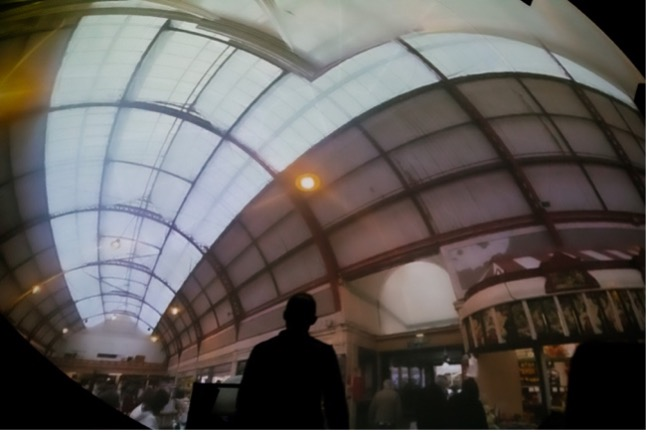
\includegraphics[width=.8\linewidth]{Images/DemVR/Findings/DomeProjection.jpg}
\end{subfigure}%
\begin{subfigure}{.5\textwidth}
  \centering
  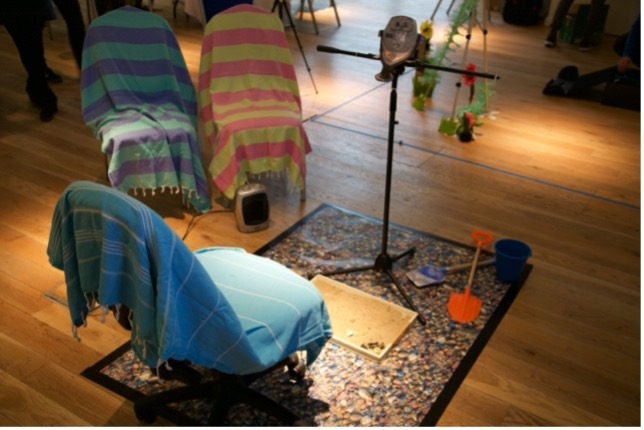
\includegraphics[width=.8\linewidth]{Images/DemVR/Findings/SensoryTideDIY.jpg}
  \label{fig:senosryTideDIY}
\end{subfigure}
\caption{Change in Sensory Tide's VR technology}
\label{fig:SensoryTideDesignProcess}
\end{figure}

With that said, even though Sensory Tide and Chatter Bench won the final prizes, they still highlighted that they struggled to construct an understanding of who the user might be. During their final presentation, Sensory Tide presented a set of personas to represent the person they were designing for: \textit{``Mary: can often get confused or lost if left alone''} (P) and \textit{``Ben: has anxiety and depression as a result of his diagnosis''} (P). Although Sensory Tide used the personas to \textit{``help us decide who we are actually designing for''} (P), for reasons similar to Chatter Bench, they found it \textit{``hard to figure out what to design because [they] can’t ask the user''} (W). This observation highlights the value teams placed on engaging with end users in the research. Here, the absent user prompted critical reflection from the team members and demonstrated key evaluation points where user feedback may encourage teams to pursue their design ideas further. 

\subsection{Making sense of dementia through design}
\label{ThemeThree:SenseofDementia}
Throughout the event, the teams' design processes opened up  ways for participants to reimagine how VR might support the person with dementia. In the pre-hackathon stage, submitted ideas helped us to form an initial picture of how prospective participants viewed dementia. For instance, Garden Life’s Ideaboard idea wanted to help people with dementia \textit{``feel more independent''}, or to \textit{``help calm the mind[s]''} (I) of people with dementia. Although multiple participants used terminology no longer accepted in best practice in dementia, such as `sufferers' and `patients' (I), the design ideas uploaded suggested these terms were not intended to stigmatise. For example, a participant from team World Share suggested ways for VR to \textit{``guide sufferers through daily basics''} (I) by having VR technology allow them to repeat tasks such as \textit{``basic cooking, making a cup of tea''} (I). Although these terms were being used early in the two day hackathon as well, through engaging in conversations with facilitators, and through introducing resources such as the DEEP Guide \citep{diaries_deep_2020},  participants adopted person-centred terms. In the same vein, many early iterations of participants’ ideas promoted `treatment', `fixing the disease' and ways for technology to improve a person's memory or other deficits. However, as highlighted in the findings above, many teams’ final ideas explore topics that go beyond dementia symptoms and related behaviour, and reimagine ways that VR experiences may support the person with dementia’s relationships with care partners, family and friends. Below, I present two sub-themes: 1) providing comfort and 2) supporting the shared experience.

\subsubsection{Providing comfort}
\label{ThemeThree:SubThemeOne}
While the facilitation and topics leaned towards broadening the conversation of dementia away from the biomedical perspective, it is important not to overlook the importance of designing for people’s impairments and abilities to use technology. Here, many design ideas took the aspect of providing comfort and educating others on dementia symptoms. For example, for team VR Hallucinate, the team reflected on Howard’s comments regarding hallucination where they wanted to tackle the \textit{``stigmatising and isolating nature''} (P) of hallucinations. Within their presentation, the team described their VR idea to provide the public, family and friends with a virtual experience of hallucinations to teach and be empathetic of the challenges faced by people with dementia. In this instance, VR Hallucinate begun to see the stigma surrounding dementia as a societal problem where friends and family may contribute to further \textit{``psychological and emotional distress for the person having the hallucination''} (P) when someone \textit{``challenges the situation''} by saying the hallucination is not real, thus drawing on socially constructed experiences of the user. \added{Likewise, this was seen between Michael and Lauren in chapter four, where Michael challenged Lauren's reality. Once challenged, it caused both of them an emotional burden. While I ended up designing media experiences that could be enjoyed by both of their realities, here, VR Hallucinate builds on this by educating family members on the matter.} Another team who took a critical approach in their design was Sensory Tides, who took inspiration from many language guides around dementia and considered what that would mean for the term `Virtual Reality' (see appendix \ref{sec:EventIdeas} for their final idea). Aware of the social challenges that people with dementia may face with defining their reality, and the concerns of a virtual simulation of a reality that may challenge the person with dementia’s understanding of reality, the team designed for continued reassurance through the technology. Instead of the term `Virtual Reality', they describe their experience as a \textit{``magical viewfinder''} (P) along with giving calm and helpful suggestions of how users may use it: either by leading the experience through the viewfinder or \textit{``lean[ing] back away from the headset and join everyone else relaxing on the [virtual] beach''} (P) (seen in figure \ref{fig:SensoryTideDesignProcess}). This demonstrates careful consideration of existing social stigma and the role of design in responding to these existing stigmas rather than permeating them. 


\begin{figure}[htp]
\centering

\includegraphics[width=.8\linewidth]{Images/DemVR/Findings/MindfulForest.png}
\caption{MindfulForest influences from Sweden dementia forest research}
\label{fig:MindFulForestResearch}
\end{figure}

Multiple teams began to question some of the more ethical and social challenges of designing for people with dementia’s abilities. For Garden Life, the team argued that \textit{``people with dementia may be fearful of VR devices''} (P), that they approached through \textit{``easing them into the experience''} by building a real-world space that replicates the VR environment by \textit{``building a comfortable garden room, featuring real plants, grass, smells, and ambident garden sounds throughout playing''} (P). \added{On the contrary, people with dementia in the both studies in chapter four never seemed fearful of VR, but rather felt silly wearing the headset in public.} Additionally, the team built a companion app that allowed the care partner to assist in guiding the person with dementia \textit{``in navigating the virtual space''} (P). In the team’s final presentation, they described how people with dementia could navigate by saying \textit{``I want to go to the flower bed area''} (P) as an alternative to using the \textit{``complicated VR joysticks''} (P). 

In similar vein, team Chatter Bench were conflicted regarding \textit{``how [to] represent the person living with dementia [in VR]''} (W). The team's idea is a `VR skype call' where both participants would be present in a 360-degree video on a bench in a park. For example, when discussing the possibilities of designing avatars for the VR environment, they worried that \textit{``the other [avatars in the environment] will look like a scary apparition or some floating smiley head''} (W). To tackle this concern, the team removed the virtual avatars and transmitted the online voices between the two users. This demonstrates the team’s consideration for mitigating discomfort for the person with dementia. Likewise, team Mindful Forest states that they originally \textit{``planned to add fantasy elements to [their] idea. But due to learning about other symptoms like hallucinations, we, therefore, had to change it to be more realistic, because we don't want to cause any problems for people with dementia''} (W). In both teams, the designers question how to virtually represent environments for people with dementia in retrospect to their potential capacity to navigate and understand the virtual environment. 

\subsubsection{Supporting the shared experience}
\label{ThemeThree:Subthemetwo}
One of the key areas of interest from the event was how designers might design shared experiences for people with dementia. Several teams’ ideas explored ways VR could provide a shared experience between family members and the person with dementia. Team Augmented World’s AR app aimed to \textit{``enhance the ability for [real-life] objects to facilitate meaningful social interaction''} (P). In Augmented World's demo, the team demonstrated a feature to augment digital media, onto an object at home (e.g. a photo frame), where the team’s intention was that people with dementia could \textit{``experience stories in a simple way, and promote interactive communication and inclusivity through shared experiences''} (P).

Here, design ideation expanded to incorporate the social home environment, inviting others into the AR experience. In Chatter Bench's presentation, the team highlighted that their shared experience might add \textit{``strain on the family and resources''} (P) in order to create the 360-degree worlds that people with dementia and care partners might want to share together – to the point that Chatter Bench presented future ideas of more social and community-led curation methods to generate a variety of environments in the \textit{``hope it will scale''} (P). This demonstrates an awareness of issues with extending caregiver duties, a sensitivity that is often overlooked in dementia care technologies. \added{Equally important, this mirrors the challenges of longevity of technology in chapter four. While families could watch the VR moments they captured, the capturing of other 360-videos remained a challenge which made scalability difficult.} Furthermore, the Chatter Bench stated that if their VR experience was implemented into a care home, then scheduling of the VR `Skype calls' needed to consider \textit{``fitting into the schedule of the care partner as well''} (W). Here \added{in the same way to chapter four,} the team show further awareness of the social context and environmental factors that informed their design. These considerations result in design that values appropriate responses to context over high-intensity VR experiences. 

With Sensory Tide, who envisioned their VR idea being placed within a care home, the team wanted to build an experience that prioritised the relationship between people with dementia and their families and friends who are visiting. In this instance, as the person with dementia controls the movement of the VR headset, this drives the experience for not only themselves, but projects what they are seeing into the outside space of the room for the family to see. \added{The idea of creating an immersive viewing space around the room resonates with the early work seen in chapter four where Karen would prompted her mother questions about what she was seeing in the VR experience.} The team's reasoning behind adding multiple sensory outputs such as \textit{``sight, sound, smell and touch''} was to \textit{``offer the user a way to engage with nature and provide props for talking points to facilitate, then, further conversation''} (P) between the person with dementia and their family members. Here, design decisions were made to support the onboarding for the person with dementia while also drawing in their family while they sat and watched their loved one take control of the virtual shared experience. Sharing new immersive experiences provides opportunity for social and therapeutic activities, thus providing new experiences for the care units.

Likewise, VR Motion designed a series of VR activities such as \textit{``songs to sing along to, guess the place, solve the riddle or even share jokes''} (P), and displayed the collaborative experiences needed to ensure continued participation within the care home. This is done through giving the staff member the responsibility as a facilitator to \textit{``pull a lever on a [VR] slot machine, which will show a random task. [Then] people with dementia and the facilitator will work together to complete the task''} (P). These examples within this sub-theme highlight tensions when designing shared experiences that are controlled or supported by others for the person with dementia. Here a focus on interdependence and the maintenance of reciprocity between family members was core to the design of the technology.

\section{Discussion}
\label{sec:Discussion}
Overall, these findings raise important considerations for future hackathons and participant involvement. This discussion section will consider the analytic findings considering existing literature on reification in design, collaborative design events, community building and meeting participants where they are. Within each subsection, I provide a set of `commitments' to mitigate stereotypes, improve recruitment processes, and ways to ensure hackathons are more inclusive and community driven. 

\subsection{Reification, experience and designing with and for stereotypes}
\label{DiscussionPartOne}
The transformation of complex individuals, groups, communities, processes, and systems into manageable constructs to inform design has long been noted in HCI. Such conceptualisations are often referred to as creating or using boundary objects, which are \textit{``entities that enhance the capacity of an idea, theory or practice to translate across culturally defined boundaries''} \cite[p.71]{fox2011boundary}, which are adaptable across application areas, but which are also solid enough to represent one `thing' or meaning across these areas too. The participants, working with an idea of their own end users, or as those dealing with instrumental cognitive problems wholly aside from the felt experience of their own dementia, were working with a boundary object – the \textit{`Person With Dementia'} - which was manageable during a weekend's design work, but may have shut down possibilities for greater creativity and wider representation. The irreducibility of individuals’ experiences means that designing with a reified idea of what it means to be a `Person with Dementia' cannot account fully for these values, needs, desires and goals. Following the work, I realised that the participants, who were working primarily from Howard’s Q\&A, as well as from artefacts and snippets from past research, were working, functionally from personas or the sort of data that might be expected from personas. The material provided, like personas as written about by \cite{marsden_stereotypes_2016}, \textit{``contribute[d] value by informing design, i.e., ha[d] a predominantly prescriptive function … they are meant to open design spaces by connecting the designers with the people they are designing for''}. 

However, such design tools and methods that abstract from the user are also prone to stereotypes – in fact, they are often built to resemble such stereotypes in order to seem more `real' by appealing to designers’ own recognition \citep{cutting_can_2019}. By appealing to this sense of recognition, however, they often `prime' certain problem areas as operationalisable for designers – for instance, a persona of someone with dementia who wanders may easily prompt a home security system or a personal alarm, where extended engagement with this person may uncover that she simply misses walking a certain stretch of a local riverbank and is content with weekly trips to do just this. Given the challenges I had with involving people with dementia in the design process, I suggest the following commitments to mitigate stereotypes for researchers and designers.

\subsubsection{Mitigating stereotyping commitment one: Thinking and talking about dementia differently}
\label{DiscussionOne:CommitTwo}
As the event went on and participants engaged with the expert facilitators, participants recognised the importance of the way they speak about dementia, with terms such as `patient', `demented' and `sufferer' being rarely used. \cite{bartlett2010broadening} draw on the power of language in which they state, \textit{``both oral and written - reflects systems of assumptions, values and beliefs''} \citep[pg.52]{bartlett2010broadening}. Despite the knock-on effects that I describe regarding the lack of people with dementia at the event, participants adopted person-centred terms through the way the facilitators and structure of the hackathon positioned people with dementia (in terms of use of language).

Additionally, \cite{bartlett2010broadening} argue that when working in the area of dementia, we must look beyond the welfare context, and instead, see all the different social identities a person with dementia might have. For instance, Chatter Bench were worried about the `strangeness' of bodily representation in VR as they felt the unfamiliarity of VR was enough to heighten the person with dementia's anxiety. Similarly, Mindful Forest decided against adding fantasy elements to their design response for fear of triggering hallucinations. My intention here is not to devalue the team's priority in safety and comfort, nor is it to suggest this is problematic as we design new technological responses. Instead, a heightened focus on risk might quash creativity, remove any room for individual differences in user experience, and further limit the expressive and aesthetic potential of the technology itself. As designers and developers continue to work in sensitive settings, researchers must continue to design approaches to provide a broader understanding and different ways of thinking about abilities. 

\subsubsection{Mitigating stereotyping commitment two: Disseminating research outputs}
\label{DiscussionOne:CommitmentThree}
One way we might mitigate stereotypical perspectives is to start disseminating dementia research into less `static' ways to offer participants new explorations into ethical and embodied topics of dementia. In the last several years, we have seen a gradual shift in disseminating dementia work, such as the theatre play Cracked, which follows a person with dementia and their family on a journey to see beyond the diagnosis. \cite{kontos_raising_2018}  designed this one-hour play that tells the story from diagnosis through to the person with dementia moving to a long-term care home. The families in the play demonstrate the changes in relationships and struggles that a diagnosis of dementia presents. Throughout the play, the director creates an immersive space for the audience to question and reflect on their assumptions, sharing and refining a more sensitive, nuanced narrative of dementia. This recent work resonates with the ongoing drive towards using film for public health and cultural awareness in educational programmes to elucidate in-class discussions \citep{botchway2017films}. 

Throughout the event, I documented the team's design processes through WhatsApp group chats, audio recordings, field notes, final idea presentations, and demos. Initially, I intended to publicly make the data publicly available to disseminate the design processes and prototypes. However, this became challenging due to unfinished prototypes and the `messiness' of design process data. Alternatively, hiring designers/filmmakers to design outputs inspired by the team’s final ideas might have disseminated the context of the event to a wider audience. Furthermore, \citeauthor{zheng2016exploring}'s \citeyear{zheng2016exploring} work on tackling dementia stigma among Chinese Americans stresses that the dissemination of information needs to be \textit{``culturally sensitive and tailored toward the values of [the] specific ethnic group''} to ensure that the message is set in a familiar setting and the audience can easily sympathise. Therefore, to get the public to engage with the more sensitive and complex topics, researchers should consider taking more creative approaches to present their work. This may be through film, theatre, zines and other creative arts to provoke similar understandings that researchers aim to gain from working alongside people with dementia.

\subsection{Facing actual reality: Shared needs and participant disinterest}
\label{DiscussionTwo}
As described in the event context and findings, the hackathon configuration gave rise to certain challenges. Prime among these was the extent to which people with dementia were meaningfully engaged in the event itself. As noted above, I tried to involve people with dementia (and their care partners) in three ways: 1) through planning workshops through a community partner with whom I've worked several times, 2) as full participants during the day itself, and 3) as participants on the online platform, Ideaboard. The former two routes failed, as no person signed up through the community partner; the latter route saw some engagement, but ultimately much less than I had hoped. Late in the planning process, I invited Howard to share his experiences and engage in a Q\&A with the participants, to ensure that the attendees had an opportunity to engage with at least one person living with the condition around which the event was centred. 

The use of Ideaboard, a participatory platform for group ideation, deserves some consideration. Part of a suite of participatory platforms launched as part of a wider research initiative aimed at including citizens in the development of services and systems for their own locality, Ideaboard took inspiration from App Movement, a similar platform that allowed limited co-design of community-commissioned apps \citep{garbett_app_2016}. However, App Movement was critiqued in a paper published in 2017 that focused on the co-design of apps for dementia services; the commissioning platform was described as \textit{``not yet nuanced enough to capture and represent aspects of the complicated experience of caring for someone with dementia or living with the condition itself''} \citep{morrissey_care_2017}. Although Ideaboard was not created solely for older users (whom I envisaged as the people living with or caring for dementia who might be interested in the hackathon), it is true that more familiar technologies might have been used in soliciting the views and opinions of participants with experiences of dementia. To mitigate these challenges in recruitment, I offer a set of commitments for recruiting and involving marginalised populations in future work:

% \subsubsection{Recruitment commitment one: Meeting your participants where they are}
% \label{DiscussionTwo:CommitOne}
% Instead of designing additional online platforms, I suggest asking participants what platforms they would like to use for engagement. Not only does this reduce development costs, but this also provides the opportunity to understand the communication processes with which participants are familiar. One approach I might have adopted would be an `Unplatformed' approach to the design of the pre-hackathon experience and recruitment stage. Unplatformed design is a model for the appropriation of social media technologies, that pays particular attention to the implications of the individual features of social media in respect to coordinating participation in specific contexts \citep{lambton-howard_unplatformed_2020}. I might have reduced barriers to engagement and ensured better representation of the views of the participants by coordinating participation on the technologies that they were already comfortable with (e.g., Twitter, Facebook, and other media platforms). Although I knew that some members of the community whom I would have liked to have reached used these platforms, I were seeking an additional ‘string to our bow’ by piloting the use of the Ideaboard platform. Nevertheless, in this case, it hindered rather than increased participation. 

% However, it should also be noted that utilising solely digital methods to facilitate recruitment and engagement could be limiting for some participants facing significant marginalisation. For instance, \cite{lazar_safe_2019} describe how even inclusive initiatives centred around the involvement of people with dementia may silence voices that offer less \textit{``polished stories''} or those who are nonverbal. \cite{dai2020making} describe that while online interactions provide an enjoyable and beneficial interaction for the person with dementia, it contributes to a burden and the need for the care partner to provide \textit{``responsive, continuous, and knowledgeable support''} \citep[pg.46:24]{hwang2020exploring}. Moreover, researcher's should consider ways to invite and involve not only people with dementia, but their care partners, friends, and family in the research process to help ensure agendas are more closely aligned with stakeholders’ priorities and desires. To this extent, participant-led research may offer understandings into new, more impactful ways the research could be of benefit to communities beyond academic publications.

\subsubsection{Recruitment commitment one: Exploring shared needs }
\label{DiscussionOne:CommitOne}
A solutionist approach in HCI has been characterised as finding a set of technological quick fixes that solve social complexities \citep{cramer2014save}. For instance, Garden Life \textit{``found it interesting that [Howard] has a pet dog''}, and so went about inscribing this already existing reality into a technological solution – they created a VR dog interaction where the user \textit{``can change its breed, colour, and name''}. This virtual representation of an enriching human-animal relationship is in stark contrast to existing research on technological approaches to designing animal companionship for older people by \cite{lazar_rethinking_2016}. In this study, older people express a need for comfort and companionship through ‘cuddling and petting live pets’ and wanting a pet that was `warm, soft', which promotes social opportunities for getting out and about and a reciprocal relationship. This is not to say that Garden Life’s idea was unsuitable, or that VR experiences cannot at all provide these sorts of qualities, but that the participants were disadvantaged by time and by lack of engagement with `real' participants – and as such, were able to provide only a shallow exemplar, which might have been much richer.

Alternatively, we might want to look towards \citeauthor{pullin2009design}'s \citeyear{pullin2009design} `resonant design' approach which starts out with designing for those who are marginalised, to then explore how these needs coincide with a broader set of users. Similar to the event where participants did not have access to iterate their ideas with the end users, designers might initially look towards designing for shared characteristics of that population, and then provide their potential users with a range of other characteristics that may not be related to their dementia. For instance, Sensory Tides' redesign of the VR headset to a seaside viewfinder to accommodate a person with dementia’s potential inexperience with VR could also open potential avenues to redesign VR headsets to be less bulky and personalised to appeal to the owner \added{which resonates with the chapter four}. Designing for a broader set of shared needs might balance the tensions between designing for abilities associated with dementia, and the more diverse individual identities to offer creative and accessible technologies that inspire new thinking rather than propose solutions.

\subsubsection{Recruitment commitment two: Fostering participation through relationships and topic training}
\label{DiscussionTwo:CommitTwo}
Within the hackathon participant recruitment, most attendees had, to some degree, technical, design and/or research skills. While I did invite care partners, social workers and practitioners, the high-level expectation of building demos or lo-fi prototypes for VR environments may have intimidated those with less technical backgrounds from participating resulting in a \textit{``limiting difference among participants''} \citep{irani_hackathons_2015}. Additionally, the technology-oriented event may have contributed to the lack of interest from people with dementia and care partners. 

In this way, I am guilty of many of the shortcomings levied against researchers who claim participatory work, yet do not involve their participants from the ground up, and don’t schedule in regular check-ins to ensure interests and priorities have not shifted. In contrast, the hackathon provided developers and designers with guides, resources, and expert facilitation on the topic of dementia that supported the building of their bespoke VR environments. Alternatively, future hackathons that invite diverse communities should consider ways to facilitate collaborative learning that would require clear indications of community outcomes to ensure participants could weigh up whether the time dedicated to supporting and training was worthwhile \citep{hayes2020inclusive}.

\subsection{Towards a new economy of collaboration for design events}
\label{DiscussionThree}
\cite{falk_olesen_10_2020} differentiate between research with, and research on hackathons, and outline a series of benefits and challenges for both, some of which have already been discussed in my account of the hackathon. One which deserves some consideration due to its frequency in other papers \citep{hope_hackathons_2019,johnson_civic_2014} is that hackathons have ‘limited sustainability and implementation of hackathon outcomes’. This paucity of workable outcomes is in stark contrast to the resources that are often ploughed into hackathons – for example, the hackathon, which drew on public funds and involved the labour of highly skilled individuals over several months, cost £5,000 to hold. While \cite{falk_olesen_10_2020} note that such events target `real-world' problems, \textit{``facilitate new research projects and publications''}, and help to \textit{``[imagine] citizenship in new ways''}, they also note that \textit{``it can be difficult for peer researchers to evaluate and build upon hackathon outcomes if the circumstances in which the outcomes were created are not well-documented''} \citep{falk_olesen_10_2020}.

This is not to say that the hackathon itself did not offer any remuneration for participants – we budgeted for their travel, their meals and their accommodation, as well as offering a prizes of £1000 and £500, which could be invested in developing their solution to a higher standard. In fact, the fast-paced nature of the hackathons, along with their high opportunity cost and valuing of technical skills over `softer' skills, belies their starting point in Silicon Valley  \citep{irani_hackathons_2015}, which remains to this day in the structure of the events, which has been described as patriarchal, capitalistic and competitive \citep{evans_disruption_2018}. When such events are predicated on `making things better' for marginalised communities with no clear pathway to actually do this; with limited participation and high barriers of engagement for these communities; with budget and university pathways to compensate the designers and developers but not the population themselves; when these events overwhelmingly focus on the problems, discrimination and indignities faced by people undergoing significant challenges: then marginalised people become the currency with which we trade. Here, I offer a set of commitments to promote more inclusive and community-driven events:

\subsubsection{Hackathon commitment one: Analysing the value of your event}
\label{DiscussionThree:CommitOne}
When applying for a grant, designing a study, or creating an event, analysing the cost-benefit, ideally with community partners, may provide insight into the events contributing value to the community. Reflecting on the lack of output the hackathon provided, preparing the event with the community may have offered us additional insights into understanding the topics of interest and the types of technologies that might be of use. For instance, while the VR hackathon stemmed from local authority interest across several years, the use of VR contradicts prior work on acknowledging technology needs to be cheap, widely accessible and be easily adapted and tailored to fit the ever-changing needs of someone living with dementia \citep{lorenz2019technology}. By analysing the cost of a project with community partners, engagement may have a) provided understanding into the type of technology the community uses, and b) gained the interest of the public who have experiences and insights into the cheaper and more accessible technologies – resulting in a greater interest in public engagement across the hackathon. Further, working with the community may have provided other alternatives for a hackathon. While I intended to understand hackathons in the dementia context, the funding provided by opportunity could have been used to support engagement between schools and care homes or contribute to funding to maintain dementia communities that are perhaps doing more for dementia than a public hackathon.

\subsubsection{Hackathon commitment two: Drawn-out phases for hackathons}
\label{DiscussionThree:CommitTwo}
Within DemVR, it was my intention to provide a set of phases that would provide a longer and drawn-out process to allow people with dementia and care partners to engage with the event. Originally, I envisioned these engagements as providing an opportunity for designers and developers to gain expert feedback and potentially collaborate with care partners and people with dementia. For instance, hackathons that are centred on a particular marginalised population may provide the space to be a learning context for not only designers and developers, but also a space for those marginalised to take part in a learning context. \cite{rosenberg2012persons} describe the challenges people with dementia face with a diagnosis and a lack of opportunities to learn technology (such as through work), due to being retired or being no longer able to work. The authors highlight that people with dementia can learn together with others to help with learning how to use technology and realise they are \textit{``not alone in being challenged by technology''} which may offer \textit{``strength, comfort, and confidence''}. Drawn-out hackathons may mirror positives seen in Game Jams where month-long cycles allow for \textit{``playtesting and refinement that short jams are not able to support''} \citep{faas2019jam}. In this way, the technology built in a hackathon does not end post-weekend, but instead, leans towards hackathons being a longer-term project that is done in the designer/developer’s spare time, where commitment to the project is driven by the relationships and learning between the communities, promoting the growing of loosely coupled, companion `communities of practice'.

Regarding design research for those of older ages or with dementia, the idea of partnering communities together – for instance, partnering a cohort of design or technology students together with a community of older people, and having both learn from one another in a mutual way – may hold promise. The UK-based ‘FixEd’ \citep{noauthor_fixperts_nodate}, has introduced a scalable learning programme called `Fixperts' that targets schools and universities to engage their students in creative problem-solving that is rooted in the communities around them – for example, a student may engage with an older neighbour to innovate simple solutions that fit into their current lives, which help to get out of a car; or another student may work with someone experiencing a time-limited disability or injury to help them navigate their college campus in a safe manner. Capitalising on the ingenuity and availability of design, technology and engineering students looking for meaningful application areas, such programmes deliver small-scale, bespoke fixes for potentially large numbers of people. Similar ideas are seen at work in programmes such as TimeBanking \citep{noauthor_hour_nodate}. Finally, given the interest in dementia as an area of interest for design and technology students, for HCI and CSCW, as well as for industry more widely, researchers should consider ways to facilitate and promote different communities to ‘partner-up’ to share knowledge and skills. 

\section{Summary}
\label{sec:Conclusion}
This chapter presents a detailed account of DemVR, a hackathon aimed at designing novel VR environments in dementia supportive contexts. The event consisted of two stages: a six-week engagement phase to support participants in proposing and refining initial ideas online, and a two-day hackathon inviting designers and domain experts to develop their ideas further. While I gained reasonable interest from designers, developers and students throughout both phases, the representation of people with dementia and their care partners was limited. I examined the structure of the event and the role this played in the struggle to involve people with dementia and their care partners. The data analysis presents insights into participants’ motivations, design approaches to accommodate the absent user and the design ideas that the teams developed to address the social context of the user. Against a background of the extant literature on reification in design, collaborative design events and dementia, the discussion provides a series of commitments for HCI and dementia research. The commitments offer insights into how we might mitigate stereotypes in constructing the end user; ways to improve recruitment to involve marginalised populations in events; and steps to promote more inclusive, community-driven events. Finally, I conclude the discussion by looking beyond hackathons to examine the role of community building to bring different communities to `partner-up' in the hope of sharing skills and knowledge to reduce stigma and provide opportunities for co-developing technical DIY products that are tailored to the person with dementia and care partner’s needs.
\added{To build upon the previous chapter, I map chapter fives insights onto the thesis research questions. (see appendix \ref{Appendix:ResearchQuestionsMapped} for overview of all chapters mapped to research questions)}

\begin{table}[htp]
    \centering
    \begin{tabular}{p{0.15\linewidth} | p{0.8\linewidth}}
      \multicolumn{2}{p{0.95\linewidth}}{\textbf{Research question one: How can we use participatory design approaches to provide meaningful and engaging experiences for people with dementia?}} 
      \\   \hline
    Chapter Five &
    \begin{itemize}
          \item Teams would rely on stakeholders' experiences of dementia to construct their understanding of dementia. Those who did not engage with other stakeholders drew on Howard's Q\&A to represent who they were designing 'for' (seen in \ref{ThemeTwo:AbsentUser}). Through the hackathon structure, participants adopted person-centred ideas to dementia by engaging with facilitators, inspiration packs and resources curated by dementia organisations (seen in \ref{ThemeThree:SenseofDementia})

      \end{itemize}
       \\ \hline
    \multicolumn{2}{p{0.95\linewidth}}{\textbf{Research question two: What are the ethical implications for people with dementia to participate in HCI research?}} 

    \\ \hline

    Chapter Five &
    \begin{itemize}
          \item Teams highlighted the difficulties in constructing who their users might be - emphasising the importance of engaging with people with dementia and the knock-on effects this had on the final ideas (seen in \ref{ThemeTwo:AbsentUser} and \ref{ThemeThree:SenseofDementia}).

          \item Some teams prioritised ways to mitigate the discomfort of VR by considering ways to navigate, use of language around `VR', and how to sensitively represent the VR environment (seen in \ref{ThemeThree:SubThemeOne}). Teams' ideas presented challenges and considerations needed for the shared VR experience (seen in \ref{ThemeThree:Subthemetwo}).

      \end{itemize}
       \\ \hline
      
    \multicolumn{2}{p{0.95\linewidth}}{\textbf{Research question three: What are the competing interests and expectations to support meaningful dialogue in dementia design research when involving multiple stakeholders - such as people with dementia, developers, designers and researchers?}} \\ \hline
     
    Chapter Five &
    \begin{itemize}
          \item While participants' motivation for taking part ranged from prize money, learning about dementia, and personal experiences, the incentives for people with dementia gave no real encouragement for taking part (seen in \ref{ThemeOne:subthemeOne}). 

          \item While chapter four demonstrated people with dementia having an appeal in participating in the research as the days were designed around their interests and needs, the hackathon overlooked the incentives for people with dementia and their care partners. As described in the commitments, if I had worked with community members, I may have provided alternatives to hackathons that felt more appropriate to people with dementia. For example, I could have taken the co-design days out of chapter four and facilitated conversations between designers, developers and people with dementia through a similar walking interview process.
      \end{itemize}
    \\ 
    
    \end{tabular}
    \caption{Chapter five mapping to research questions}
    \label{chapterFiveRQ}
\end{table}


\pagebreak
\added{From the previous two chapters, they have been several ethical implications that I have encountered when inviting people with dementia to participate in research and design. In chapter four, participation was challenging for one particular family where the family member with dementia could not provide verbal consent at the time of the study, which questions the infrastructures that often uphold research - such as ethical review boards. Not participating can have multiple knock-on effects on technology design, where designers and developers struggle to tailor the technology to the user. Similarly, in the hackathon, teams found it challenging to construct who their users might be due to not being able to iterate on their idea through feedback and testing with the end user. Furthermore, while chapter four reported on the different incentives for people with dementia to get involved in the study, the hackathon overlooked the incentives for care partners and people with dementia where there was no real encouragement to participate.} To respond to the ethical concerns faced in chapters four and five, the following chapter examines the impact of research ethics on participatory approaches in dementia from a researcher's perspective. The chapter presents a study inviting 22 HCI dementia researchers to share their experiences into the ethical considerations required when carrying out design research with people with dementia.



